\documentclass[a4paper]{article}

% CJK support: prefer ctex, fallback to XeTeX native line breaking
\IfFileExists{ctex.sty}{
  \usepackage[fontset=fandol]{ctex}
}{
  % Fallback for minimal TeX installs (e.g. MacTeX Basic, TeX Live scheme-basic)
  % without ctex/xeCJK. Uses XeTeX's built-in CJK line breaking.
  \usepackage{fontspec}
  \XeTeXlinebreaklocale "zh"
  \XeTeXlinebreakskip = 0pt plus 1pt
  \IfFontExistsTF{Songti SC}{\setmainfont{Songti SC}}{%
    \IfFontExistsTF{Noto Serif CJK SC}{\setmainfont{Noto Serif CJK SC}}{}%
  }
  \IfFontExistsTF{Heiti SC}{\setsansfont{Heiti SC}}{%
    \IfFontExistsTF{Noto Sans CJK SC}{\setsansfont{Noto Sans CJK SC}}{}%
  }
}

% Basic packages
\usepackage{amsmath, amssymb}
\usepackage{graphicx}
\usepackage[margin=2.5cm]{geometry}
\emergencystretch=3em
\usepackage[most]{tcolorbox}
\usepackage{etoolbox}
\usepackage{listings}
\usepackage{hyperref}
\usepackage{booktabs}
\usepackage{array}
\usepackage{subcaption}
\usepackage{float}
\usepackage{tikz}
\IfFileExists{pgfplots.sty}{
    \usepackage{pgfplots}
    \pgfplotsset{compat=1.18}
}{}

% ===== Highlight boxes =====
\newtcolorbox{knowledgebox}[1]{
    enhanced, colback=blue!5!white, colframe=blue!75!black, colbacktitle=blue!75!black,
    coltitle=white, fonttitle=\bfseries, title={#1}, attach boxed title to top left={yshift=-2mm, xshift=2mm},
    boxrule=1pt, sharp corners
}

\newtcolorbox{importantbox}[1]{
    enhanced, colback=yellow!10!white, colframe=yellow!80!black, colbacktitle=yellow!80!black,
    coltitle=black, fonttitle=\bfseries, title={#1}, sharp corners
}

\newtcolorbox{warningbox}[1]{
    enhanced, colback=red!5!white, colframe=red!75!black, colbacktitle=red!75!black,
    coltitle=white, fonttitle=\bfseries, title={#1}, sharp corners
}

\newtcolorbox{practicebox}[1]{
    enhanced, colback=black!3!white, colframe=black!75, colbacktitle=black!75,
    coltitle=white, fonttitle=\bfseries, title={#1}, sharp corners
}

% ===== Code listings =====
\lstset{
    basicstyle=\ttfamily\small,
    keywordstyle=\color{blue},
    stringstyle=\color{red!60!black},
    commentstyle=\color{green!60!black},
    breaklines=true,
    frame=single,
    numbers=left,
    numberstyle=\tiny\color{gray},
    captionpos=b,
    extendedchars=false
}

% ===== Figure provenance and unit macros =====
% \vtag goes inside \caption{...}; \srcnote{MM:SS--MM:SS} follows the figure environment.
\newcommand{\vtag}{\protect\footnotemark}
\newcommand{\srcnote}[1]{\footnotetext{视频画面时间区间：#1。若为裁剪图，时间区间仍对应原视频画面。}}
% Units work in text and math mode; never hand-write $^\circ$ or \AA inside \mathrm.
\newcommand{\degC}{\ensuremath{^{\circ}\mathrm{C}}}
\newcommand{\um}{\ensuremath{\mu\mathrm{m}}}
\newcommand{\nm}{\ensuremath{\mathrm{nm}}}
\newcommand{\angstrom}{\ensuremath{\text{\AA}}}

% ===== Front-page metadata =====
% Fill these in when generating notes.
\newcommand{\notetitle}{插值与拟合}
\newcommand{\notesubtitle}{GAMES001 图形学中的数学 · 第 6 集：线性与多项式插值、样条、厄米插值、基函数、高维插值、最小二乘、MLS 与 RANSAC}
\newcommand{\noteauthors}{根据 GAMES-Webinar 直播录像整理（阮良旺 主讲）}
\newcommand{\notedate}{2024年4月8日（直播）}
\newcommand{\videochannel}{GAMES-Webinar（哔哩哔哩）}
\newcommand{\videopublishdate}{2024年3月6日（合集）}
\newcommand{\videoduration}{1小时32分36秒}
\newcommand{\videourl}{https://www.bilibili.com/video/BV1MF4m1V7e3/?p=6}
\newcommand{\videocoverpath}{cover.jpg}

\begin{document}

% ===== Title page =====
\begin{titlepage}
\centering
{\Large 课程笔记\par}
\vspace{1.2cm}
{\huge\bfseries \notetitle\par}
\ifdefempty{\notesubtitle}{}{
\vspace{0.3cm}
{\large \notesubtitle\par}
}
\vspace{0.5cm}
{\large \noteauthors\par}
\vspace{0.3cm}
{\large \notedate\par}
\vspace{1.0cm}

\ifdefempty{\videocoverpath}{
{\small 请在生成笔记时填入视频封面图的本地路径。\par}
}{
\includegraphics[width=0.82\textwidth,height=0.40\textheight,keepaspectratio]{\videocoverpath}\par
}

\vfill
\begin{tcolorbox}[width=0.9\textwidth, colback=black!2!white, colframe=black!60, sharp corners]
\textbf{视频作者/频道}：\videochannel\par
\textbf{发布日期}：\videopublishdate\par
\textbf{视频时长}：\videoduration\par
\textbf{视频链接}：
\ifdefempty{\videourl}{
未填写
}{
\href{\videourl}{\nolinkurl{\videourl}}
}
\end{tcolorbox}
\end{titlepage}

\tableofcontents
\newpage

%% --- 正文内容开始 --- %%

\section{插值与拟合：两个不同的问题}

第六讲由阮良旺主讲，主题是插值（interpolation）与拟合（curve fitting）。讲者开场说明，原本打算这一讲把“采样”也一起讲完，但采样的内容与下一讲的傅里叶变换关系更密切，一次讲太多也容易贪多嚼不烂，所以这一讲只讲插值和拟合，因为这两部分本身的内容已经不少。

在讲具体方法之前，首先要区分这两个概念。它们都从一组离散的采样点出发，想得到一条连续的曲线，但定义非常清楚地不同：\textbf{插值}要求曲线一定经过所有采样点；\textbf{拟合}不要求经过采样点，只要求曲线整体上尽量接近数据。两者对应两种不同的场景：插值通常假定采样点本身是准确的，我们只是想补出采样点之间缺失的信息；拟合则假定数据带有噪声，或者我们事先知道数据服从某种规律，只想找到那条规律本身。

\noindent\begin{minipage}{\textwidth}
\begin{figure}[H]
\centering
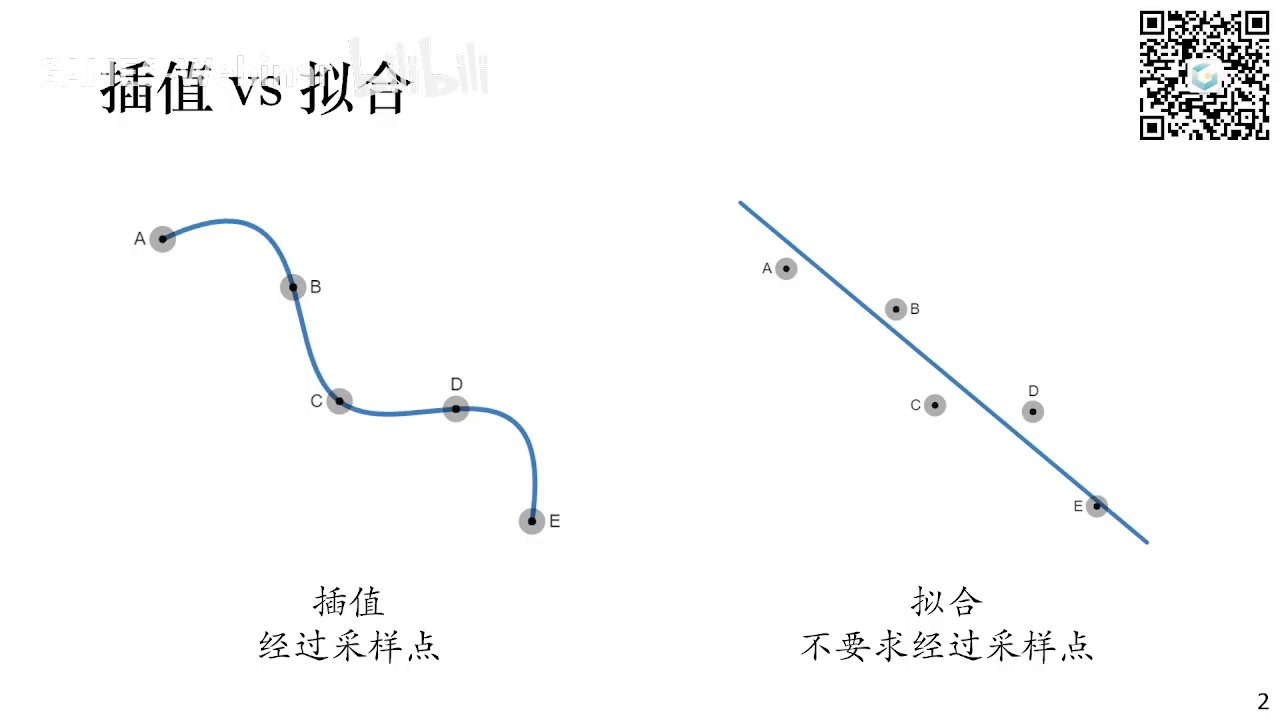
\includegraphics[width=0.92\textwidth]{figures/fig_01_interp_vs_fit.jpg}
\caption{插值经过所有采样点，拟合不要求经过采样点\vtag}
\end{figure}
\srcnote{00:01:30--00:01:45}
\end{minipage}


\begin{importantbox}{本讲的主线}
本讲前大半讲插值：从线性插值、多项式插值出发，看到龙格现象，引出样条插值；再用三阶厄米插值换取局部性，用“基函数”的视角统一各种插值方法；然后把一维插值推广到曲线、三角形、多边形、像素和点云。后一部分讲拟合：最小二乘法、移动最小二乘，以及适用于大量离群点的 RANSAC。比较各种方法时始终关注三个指标：\textbf{连续性}、\textbf{计算复杂性}和\textbf{局部性}。
\end{importantbox}

\section{一维插值：从线性到多项式}

\subsection{线性插值与连续性}

最简单的插值是线性插值（linear interpolation）。已知两个点 $(x_0,y_0)$ 和 $(x_1,y_1)$，要补出它们之间的信息，最自然的做法就是在两点之间画一条线段。按斜率写出直线方程，再整理成两端值的加权和：
\[
y=y_0+\frac{y_1-y_0}{x_1-x_0}(x-x_0)=\frac{x_1-x}{x_1-x_0}y_0+\frac{x-x_0}{x_1-x_0}y_1 .
\]
如果令 $x$ 在线段 $[x_0,x_1]$ 中的比率为 $t$，就得到更常见的写法
\[
y=(1-t)y_0+ty_1,\qquad t=\frac{x-x_0}{x_1-x_0}.
\]
$t$ 取零时 $y=y_0$，取一时 $y=y_1$，中间按比例过渡。

\noindent\begin{minipage}{\textwidth}
\begin{figure}[H]
\centering
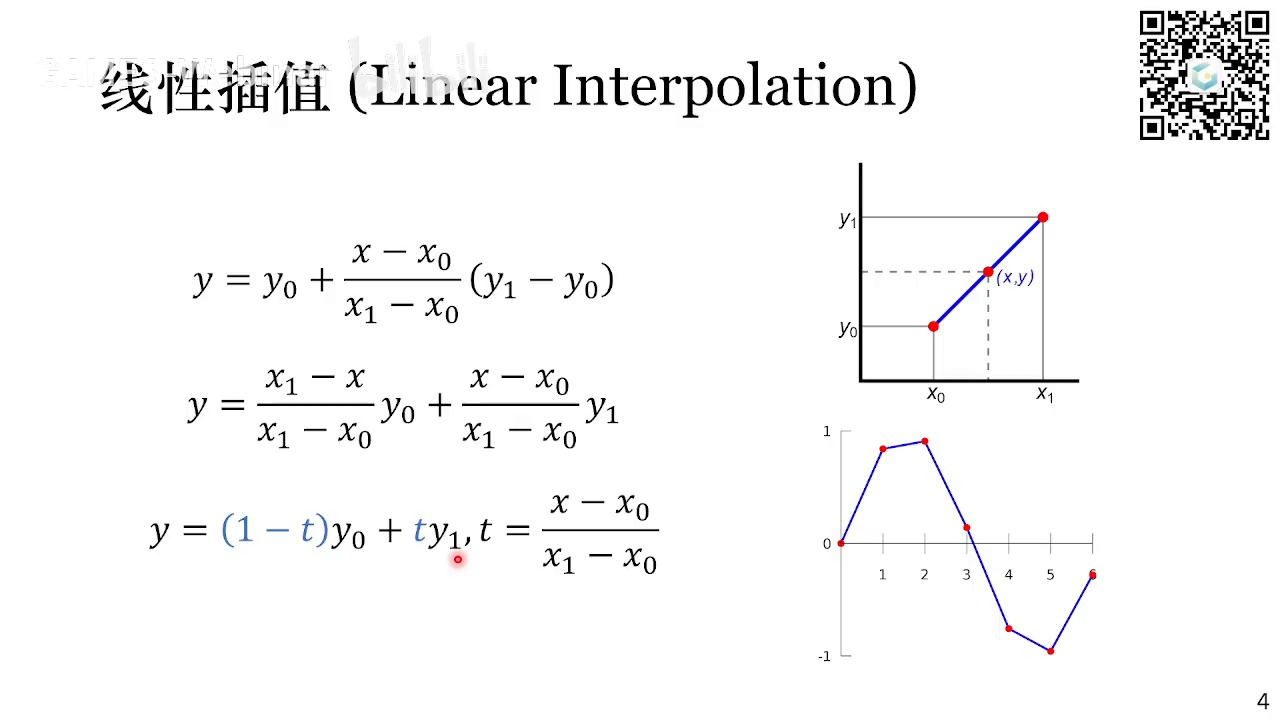
\includegraphics[width=0.92\textwidth]{figures/fig_02_linear.jpg}
\caption{线性插值：两点之间连线段，写成 $(1-t)y_0+ty_1$\vtag}
\end{figure}
\srcnote{00:03:15--00:03:30}
\end{minipage}


把很多个点依次用线段连起来，得到的折线没有断点，但在每个采样点处导数会发生跳变。这种“函数值连续而导数不连续”的情况称为 $C^0$ 连续。一般地，若曲线直到 $k$ 阶导数都连续，就称为 $C^k$ 连续。线性插值满足了最基本的连续要求；如果对光滑性有更高的要求，比如动画中的运动轨迹不能突然“拐弯”，线性插值就不够用了。

\noindent\begin{minipage}{\textwidth}
\begin{figure}[H]
\centering
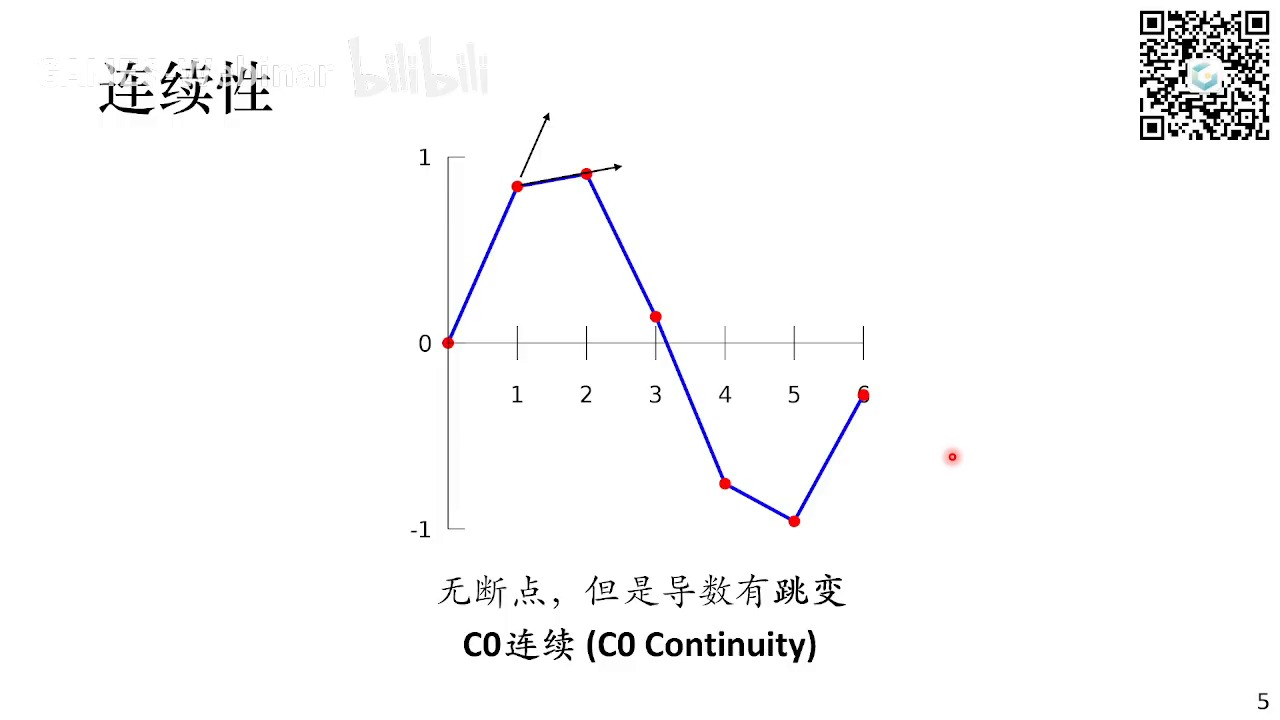
\includegraphics[width=0.92\textwidth]{figures/fig_03_continuity.jpg}
\caption{$C^0$ 连续：没有断点，但导数在采样点处跳变\vtag}
\end{figure}
\srcnote{00:04:00--00:04:15}
\end{minipage}


\subsection{二阶插值与范德蒙矩阵}

更高一阶的做法是用二次函数 $y=ax^2+bx+c$ 去经过三个点 $(x_i,y_i)$，$i=0,1,2$。三个插值条件写成矩阵方程
\[
\begin{pmatrix}x_0^2&x_0&1\\x_1^2&x_1&1\\x_2^2&x_2&1\end{pmatrix}
\begin{pmatrix}a\\b\\c\end{pmatrix}=
\begin{pmatrix}y_0\\y_1\\y_2\end{pmatrix}.
\]
左边的矩阵长得非常有规律，每一行都是同一个数的各次幂，称为\textbf{范德蒙矩阵}（Vandermonde matrix）。只要三个 $x_i$ 互不相同，它就可逆。解出系数后经过变换，可以把二次函数写成另一种形式：
\[
y=\frac{(x-x_1)(x-x_2)}{(x_0-x_1)(x_0-x_2)}y_0+\frac{(x-x_0)(x-x_2)}{(x_1-x_0)(x_1-x_2)}y_1+\frac{(x-x_0)(x-x_1)}{(x_2-x_0)(x_2-x_1)}y_2 .
\]
这个式子很容易验证：代入 $x=x_0$，第一项的分子变成 $(x_0-x_1)(x_0-x_2)$，与分母相同，系数为一；第二、三项里都有因子 $x-x_0$，等于零。所以 $y(x_0)=y_0$，另外两个点同理。

\noindent\begin{minipage}{\textwidth}
\begin{figure}[H]
\centering
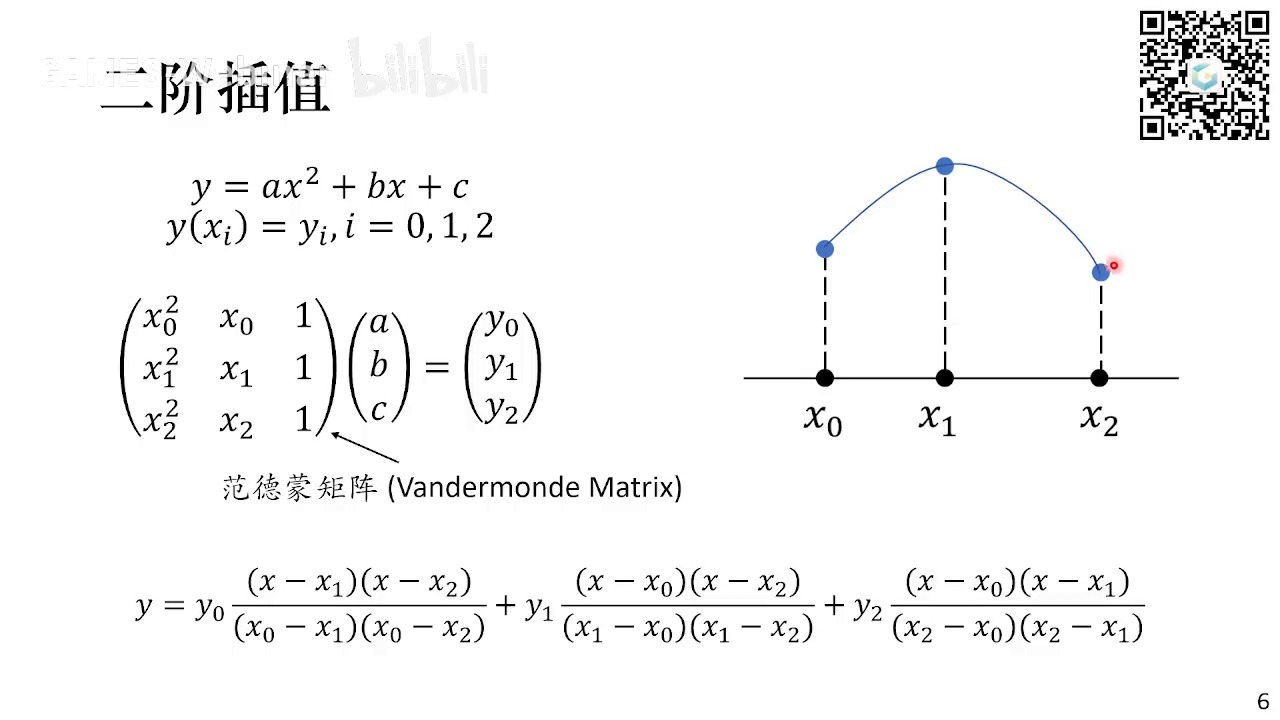
\includegraphics[width=0.92\textwidth]{figures/fig_04_quadratic.jpg}
\caption{二阶插值：范德蒙矩阵方程与等价的乘积形式\vtag}
\end{figure}
\srcnote{00:07:30--00:07:45}
\end{minipage}


\subsection{多项式插值与拉格朗日多项式}

推广到一般情况：一共有 $n+1$ 个数据点 $(x_0,y_0),\dots,(x_n,y_n)$，寻找多项式 $y(x)=a_0+a_1x+\cdots+a_nx^n$ 经过所有点。为什么是 $n$ 次？因为每个点给出一个方程，$n+1$ 个方程恰好确定 $n+1$ 个系数。仿照二阶的形式，直接写出
\[
y=\sum_{j=0}^ny_j\,L_j(x),\qquad L_j(x)=\prod_{i=0,\,i\neq j}^{n}\frac{x-x_i}{x_j-x_i}.
\]
连乘对 $i\neq j$ 进行，共 $n$ 个因子，所以 $L_j$ 是 $n$ 次多项式，称为\textbf{拉格朗日多项式}。它最重要的性质是
\[
L_j(x_k)=\prod_{i\neq j}\frac{x_k-x_i}{x_j-x_i}=\delta_{jk}=\begin{cases}1,&k=j\\0,&k\neq j\end{cases}
\]
当 $k=j$ 时每个因子的分子分母相同；当 $k\neq j$ 时，连乘中一定有一项 $i=k$，分子为零。于是 $y(x_k)=\sum_jy_j\delta_{jk}=y_k$。这个公式直接给出了插值多项式的形式，只要把 $x$ 代进去，就能得到任意点的函数值，不需要先解方程。

\noindent\begin{minipage}{\textwidth}
\begin{figure}[H]
\centering
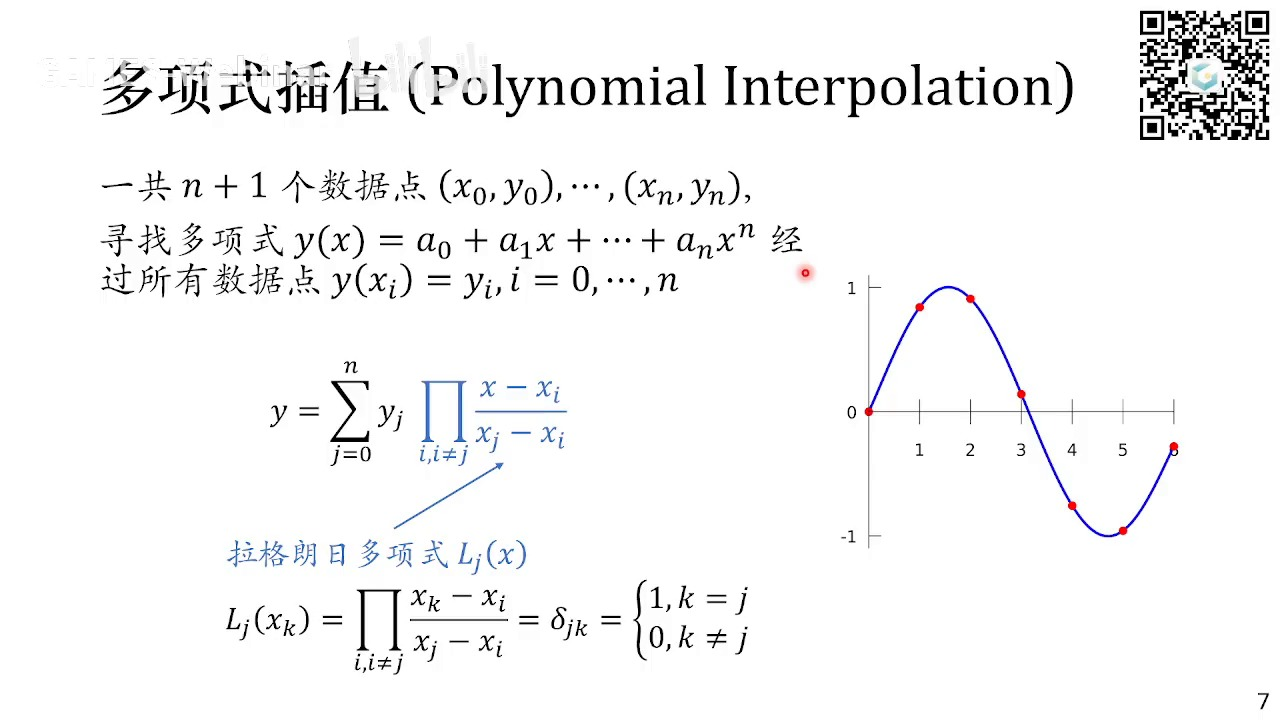
\includegraphics[width=0.92\textwidth]{figures/fig_05_polynomial.jpg}
\caption{多项式插值：$n+1$ 个点确定 $n$ 次多项式，拉格朗日多项式满足 $L_j(x_k)=\delta_{jk}$\vtag}
\end{figure}
\srcnote{00:12:45--00:13:00}
\end{minipage}


\begin{knowledgebox}{“找规律”题的另一个答案}
讲者举了一个知乎上流行的例子：数列 20、22、25、30、37，下一项是多少？选项是 47、49、55、81。按“差为质数”的思路，大概会选某一个答案；但用多项式插值的观点，四个选项其实\emph{都对}：把已知的五项和任意一个候选值作为六个点，拉格朗日公式一定能给出一个经过这六个点的五次多项式。这个例子说明，只给有限个采样点时，插值结果完全取决于我们选择的函数族；“规律”是假设出来的，不是数据本身唯一决定的。
\end{knowledgebox}

\noindent\begin{minipage}{\textwidth}
\begin{figure}[H]
\centering

\includegraphics[width=0.92\textwidth]{figures/fig_06_sequence.jpg}
\caption{“如何寻找数列下一项”：用多项式插值，任何候选答案都能被解释\vtag}
\end{figure}
\srcnote{00:14:45--00:15:00}
\end{minipage}


\subsection{龙格现象}

多项式插值有一个严重的问题，称为\textbf{龙格现象}（Runge's phenomenon）。课件中黑色的曲线是真实函数（ground truth），在上面采样 10 个点，用多项式插值出一条曲线。结果插出来的多项式在中间部分与真实曲线吻合，但在两端剧烈振荡，偏离得非常远。尽管多项式曲线处处光滑，结果却可能非常振荡。

为什么会振荡？讲者的解释是：出现这么多次振荡，一定是因为多项式的阶数足够高。二次多项式只有一个极值点，三次多项式最多有两个；点越多，多项式阶数越高，可能出现的极值点越多。高阶多项式为了同时经过所有点，只能在点与点之间来回摆动。

\noindent\begin{minipage}{\textwidth}
\begin{figure}[H]
\centering
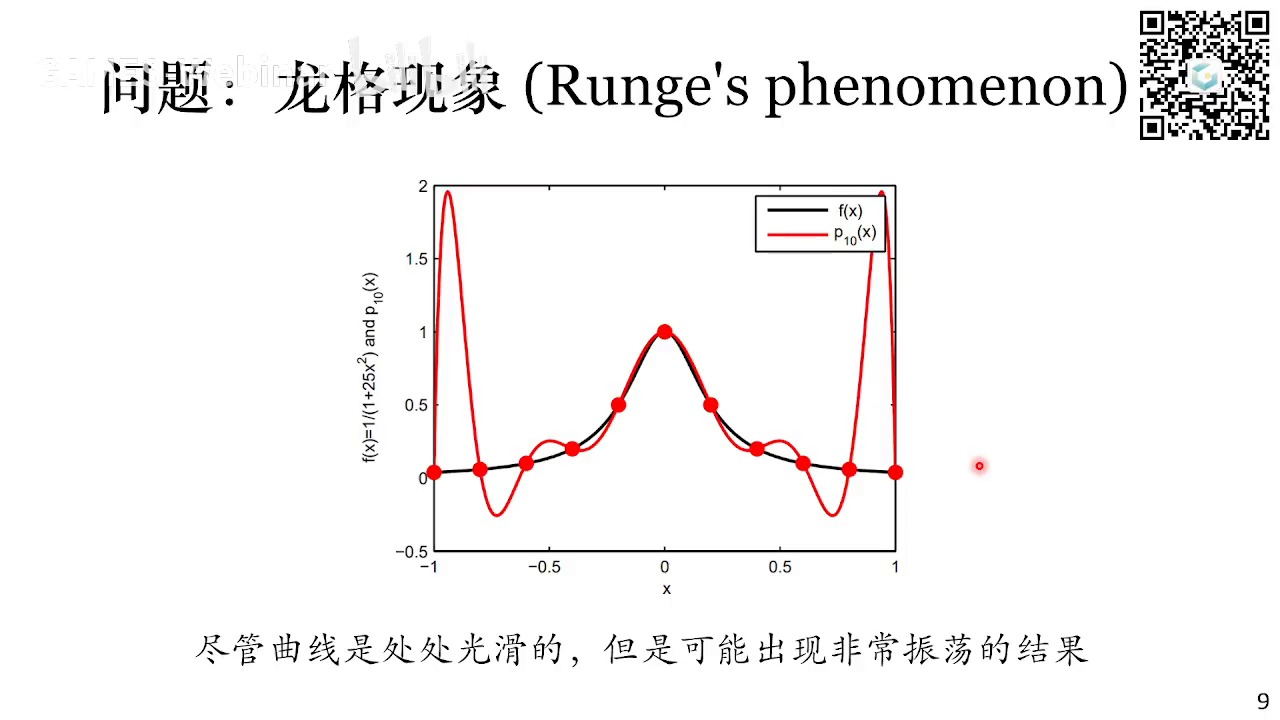
\includegraphics[width=0.92\textwidth]{figures/fig_07_runge.jpg}
\caption{龙格现象：高阶多项式插值在区间两端剧烈振荡\vtag}
\end{figure}
\srcnote{00:16:30--00:16:45}
\end{minipage}


\begin{warningbox}{点越多不一定越好}
直觉上采样点越多，插值应该越准；但对等距采样的全局多项式插值，点越多阶数越高，两端的振荡反而越严重。所以实际中几乎不用高阶的全局多项式插值，而是改用分段的低阶多项式，也就是下面的样条。
\end{warningbox}

\section{样条插值}

\subsection{思路：拼接低阶多项式}

解决龙格现象的方法是\textbf{样条插值}（spline interpolation）：不用一个高阶多项式经过所有点，而是在相邻点之间各用一段低阶多项式，再把它们拼接起来。最开始介绍的线性插值其实就是一种样条插值，只是每段多项式的阶数太低，只有一次，每一段都是直线。

\noindent\begin{minipage}{\textwidth}
\begin{figure}[H]
\centering
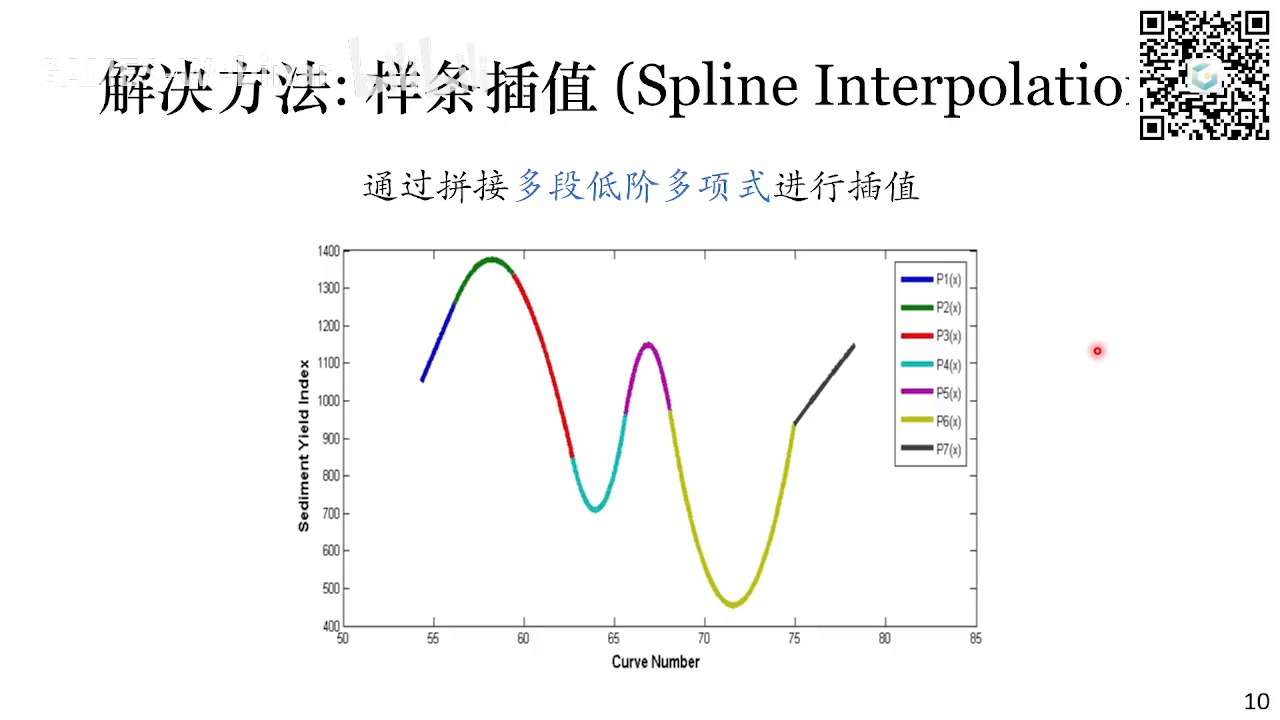
\includegraphics[width=0.92\textwidth]{figures/fig_08_spline_idea.jpg}
\caption{样条插值：拼接多段低阶多项式进行插值\vtag}
\end{figure}
\srcnote{00:17:45--00:18:00}
\end{minipage}


\subsection{二阶样条}

二阶样条（quadratic spline）中每一段都是二次函数。$n+1$ 个数据点共有 $n$ 个区间，第 $i$ 段为 $a_ix^2+b_ix+c_i$，共 $3n$ 个未知数。条件如下。

\textbf{插值条件}：区间 $i$ 的二次函数要经过两个端点
\[
a_ix_i^2+b_ix_i+c_i=y_i,\qquad a_ix_{i+1}^2+b_ix_{i+1}+c_i=y_{i+1},
\]
共 $2n$ 个方程。这保证了曲线连续，至少不比线性插值差。

\textbf{导数光滑条件}：在每个内部数据点 $x_i$，左右两段的导数相同
\[
2a_{i-1}x_i+b_{i-1}=2a_ix_i+b_i ,
\]
共 $n-1$ 个方程。

方程数比未知数少一个：$3n-2n-(n-1)=1$。剩下这个自由度需要人为指定，例如强行规定第一段是线性函数，即 $a_0=0$。

\noindent\begin{minipage}{\textwidth}
\begin{figure}[H]
\centering
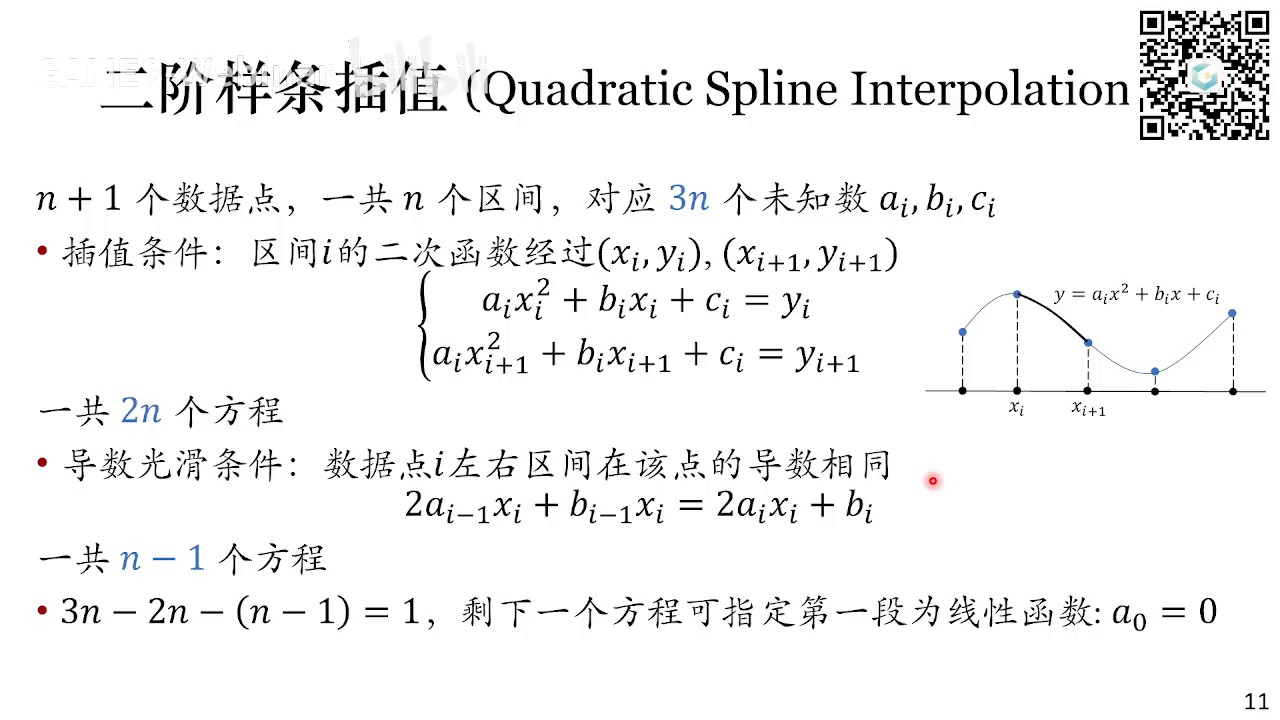
\includegraphics[width=0.92\textwidth]{figures/fig_09_quadratic_spline.jpg}
\caption{二阶样条：$3n$ 个未知数，$2n$ 个插值条件与 $n-1$ 个导数条件，再指定 $a_0=0$\vtag}
\end{figure}
\srcnote{00:20:15--00:20:30}
\end{minipage}


二阶样条的结果是一阶导数连续的（$C^1$），但二阶导数不连续，因为并没有要求各段的 $a_i$ 相同。它还有两个缺点：第一，需要联立求解大小为 $3n$ 的矩阵方程，没有显式解，速度慢；第二，每个数据点都会影响全局的插值结果。讲者举例说，把 $x_i$ 处的点稍微动一下，可能会影响到最末尾那一段曲线的形状，这就是局部性不好。

\begin{importantbox}{为什么局部性重要}
在交互式应用中，用户拖动一个控制点，只希望附近的曲线跟着变；如果整条曲线都随之抖动，编辑就无从下手。在动画中，修改某一帧的关键姿态也不应影响很远处的动作。局部性还意味着计算可以局部进行：只需重算受影响的几段，而不必每次重新求解整个方程组。这就是为什么讲者在比较插值方法时，始终把局部性与连续性、复杂性并列为三个指标。
\end{importantbox}

\noindent\begin{minipage}{\textwidth}
\begin{figure}[H]
\centering
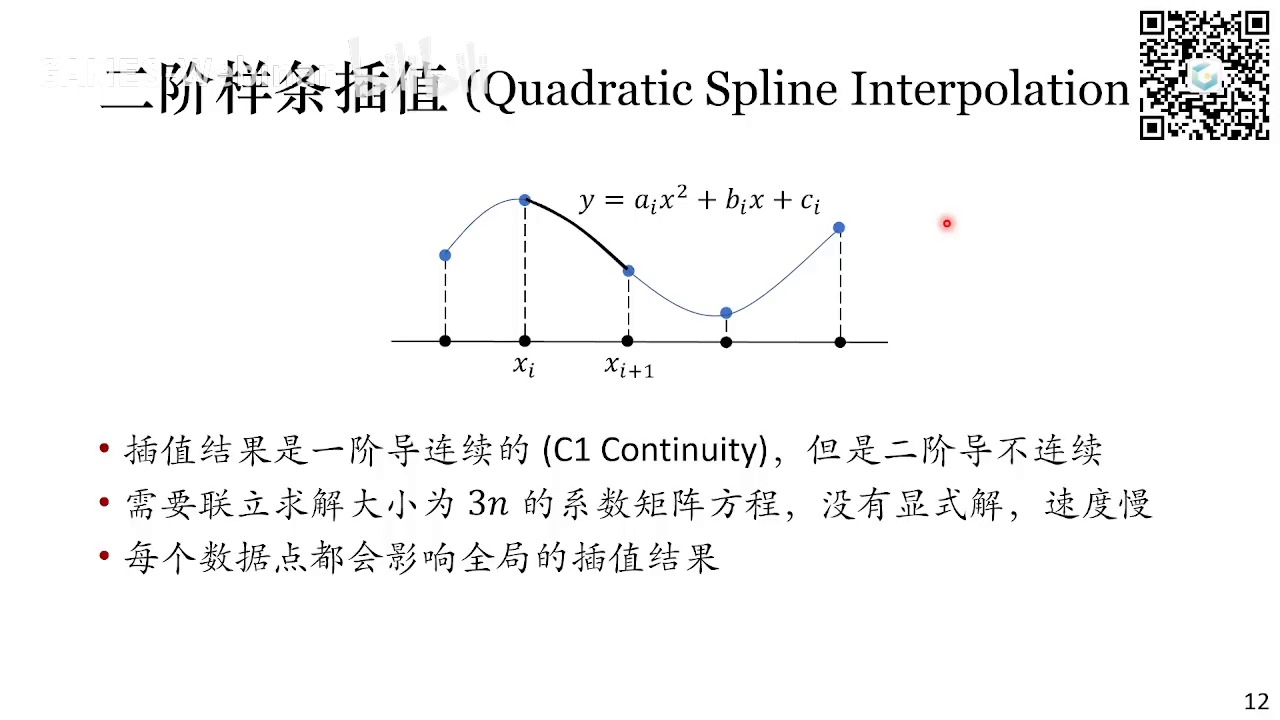
\includegraphics[width=0.92\textwidth]{figures/fig_10_quadratic_spline_result.jpg}
\caption{二阶样条的结果：$C^1$ 连续，但需要解全局方程，局部性差\vtag}
\end{figure}
\srcnote{00:22:30--00:22:45}
\end{minipage}


\subsection{三阶样条}

三阶样条（cubic spline）可以用类似的方式定义。$n$ 个区间共 $4n$ 个未知数；条件有 $2n$ 个函数值连续条件、$n-1$ 个一阶导数连续条件、$n-1$ 个二阶导数连续条件，还差 2 个，需要额外指定，比如规定两端的二阶导数为零（自然样条）。好处是插值结果二阶导数连续（$C^2$），更光滑；坏处与二阶情况一样，需要求解系数矩阵方程，单个数据点会影响全局插值结果。

\noindent\begin{minipage}{\textwidth}
\begin{figure}[H]
\centering
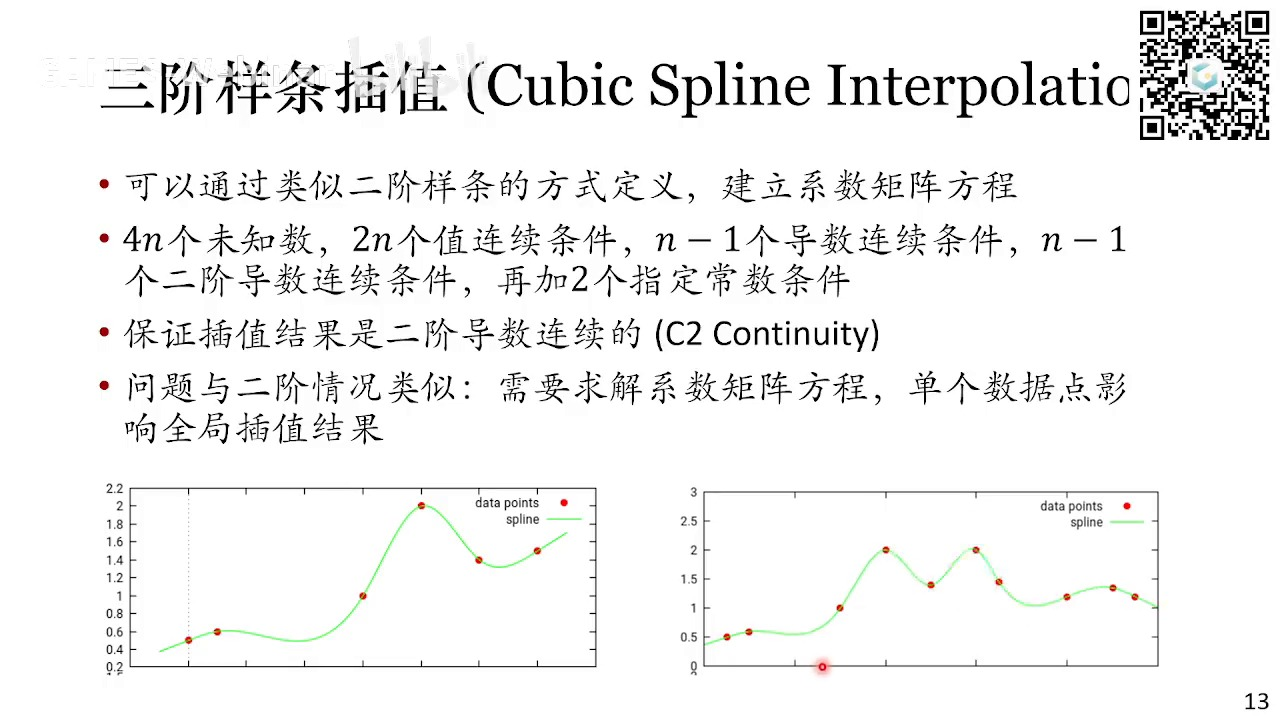
\includegraphics[width=0.92\textwidth]{figures/fig_11_cubic_spline.jpg}
\caption{三阶样条：$4n$ 个未知数，保证 $C^2$ 连续\vtag}
\end{figure}
\srcnote{00:24:30--00:24:45}
\end{minipage}


\begin{knowledgebox}{三对角方程的快速解法}
样条插值的方程虽然要整体求解，但矩阵结构很好。以三阶样条为例，若以各点处的二阶导数为未知数，方程组的系数矩阵是对称三对角且对角占优的，只有主对角线和两条副对角线非零。这类方程可以用追赶法（Thomas 算法）在 $O(n)$ 时间内求解，远快于一般的高斯消元。讲者推荐了 GAMES102 的学习材料作为参考。
\end{knowledgebox}

\noindent\begin{minipage}{\textwidth}
\begin{figure}[H]
\centering
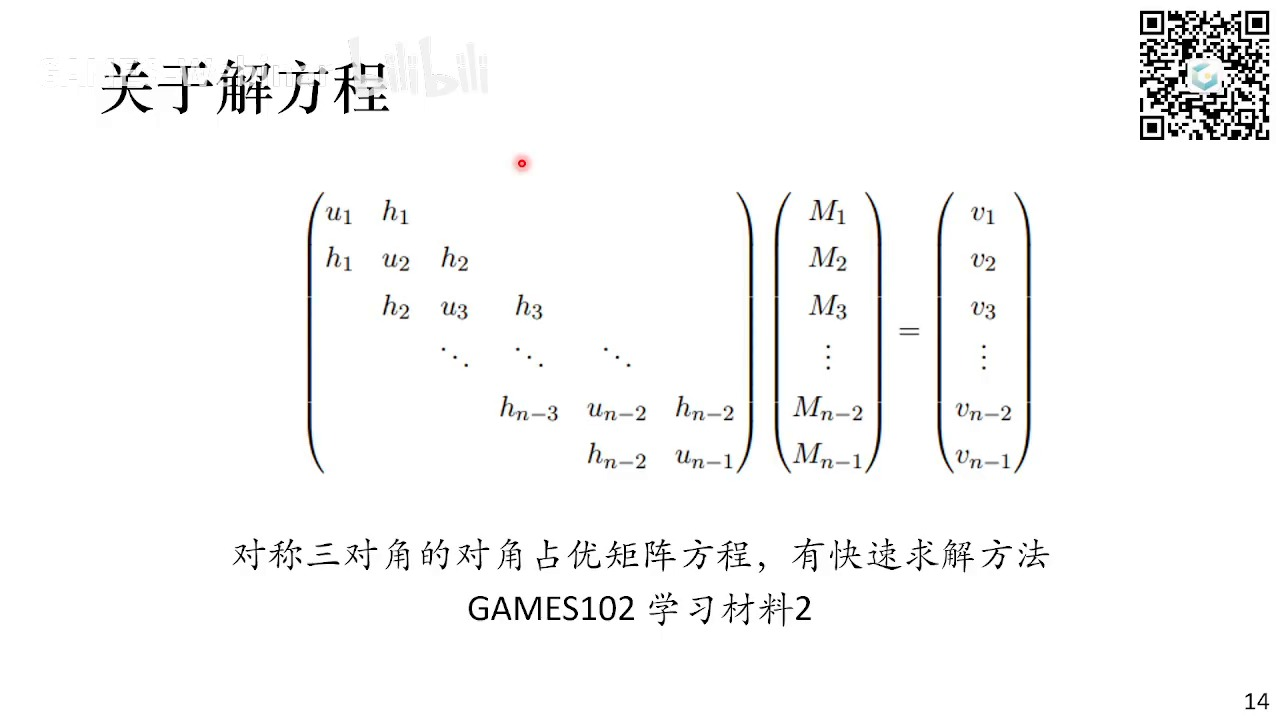
\includegraphics[width=0.92\textwidth]{figures/fig_12_tridiagonal.jpg}
\caption{样条方程是对称三对角的对角占优矩阵方程，有快速解法\vtag}
\end{figure}
\srcnote{00:25:30--00:25:45}
\end{minipage}


\section{三阶厄米插值}

\subsection{用导数换局部性}

三阶厄米插值（cubic Hermite interpolation）的名字与三阶样条很像，有些地方也称为厄米样条插值。它的思路是：\emph{放弃二阶导数连续的要求}，让插值获得更好的局部性。尽管每段仍是三次多项式，结果只保证一阶连续。

每段 $y(x)=ax^3+bx^2+cx+d$ 有 4 个系数。除了两个端点的函数值条件 $y(x_0)=y_0$、$y(x_1)=y_1$，再增加两个导数条件 $y'(x_0)=m_0$、$y'(x_1)=m_1$，恰好 4 个方程。用 $t=(x-x_0)/(x_1-x_0)$ 改写，结果很漂亮：
\[
y=(2t^3-3t^2+1)y_0+(t^3-2t^2+t)m_0(x_1-x_0)+(-2t^3+3t^2)y_1+(t^3-t^2)m_1(x_1-x_0).
\]
它是 $t$ 的三次多项式，因而也是 $x$ 的三次多项式，只是换了写法。导数项乘以 $x_1-x_0$ 来自链式法则：$\mathrm dy/\mathrm dx=(\mathrm dy/\mathrm dt)/(x_1-x_0)$。

\noindent\begin{minipage}{\textwidth}
\begin{figure}[H]
\centering
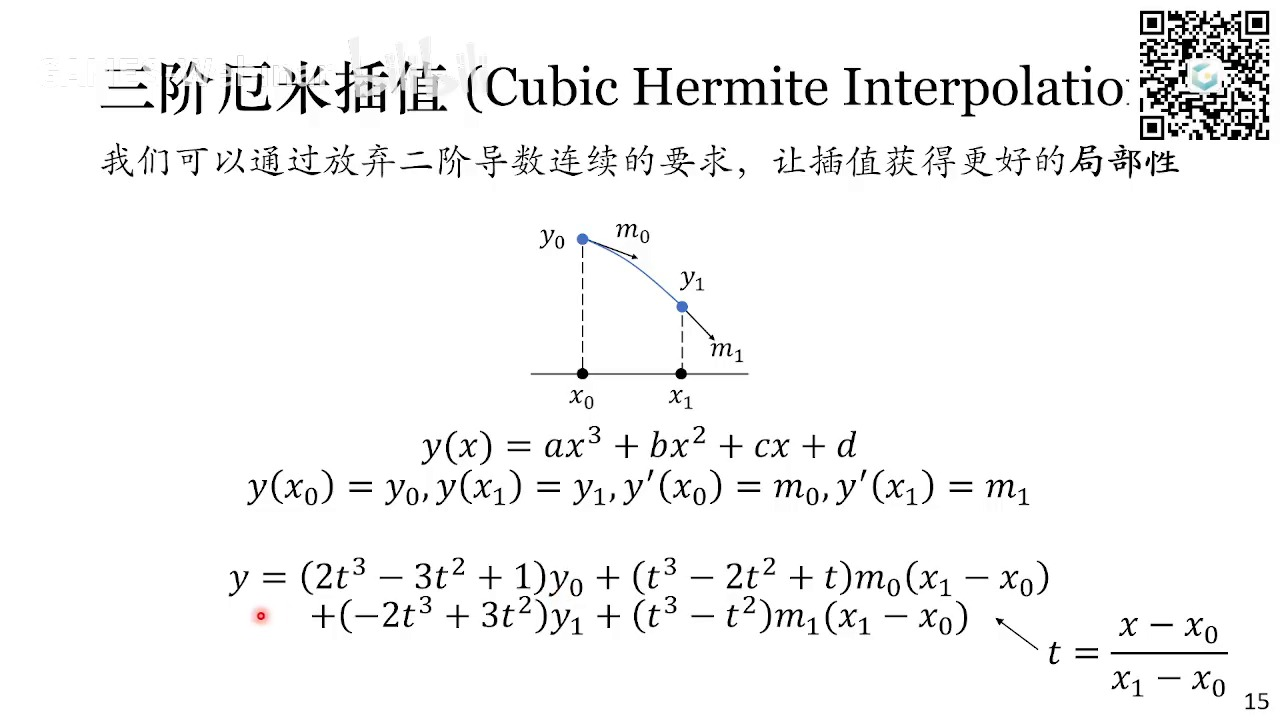
\includegraphics[width=0.92\textwidth]{figures/fig_13_hermite.jpg}
\caption{三阶厄米插值：用端点函数值和导数确定每段三次多项式\vtag}
\end{figure}
\srcnote{00:29:15--00:29:30}
\end{minipage}


\subsection{厄米基函数}

上式中 $y_0,m_0,y_1,m_1$ 前面的四个多项式称为\textbf{厄米基函数}，记为 $h_{00},h_{10},h_{01},h_{11}$。它们在端点的取值和导数满足
\[
\begin{aligned}
h_{00}(0)&=1,\ h_{00}'(0)=0,\ h_{00}(1)=0,\ h_{00}'(1)=0; &\quad h_{10}(0)&=0,\ h_{10}'(0)=1,\ h_{10}(1)=0,\ h_{10}'(1)=0;\\
h_{01}(0)&=0,\ h_{01}'(0)=0,\ h_{01}(1)=1,\ h_{01}'(1)=0; &\quad h_{11}(0)&=0,\ h_{11}'(0)=0,\ h_{11}(1)=0,\ h_{11}'(1)=1.
\end{aligned}
\]
每个基函数只“负责”一个量：比如 $h_{00}$（红线）在 $t=0$ 处取一、在 $t=1$ 处取零，两端导数都为零；$h_{01}$（深蓝线）与它对称。$h_{10}$ 只在 $t=0$ 处导数为一，其余三个量都为零。

\noindent\begin{minipage}{\textwidth}
\begin{figure}[H]
\centering
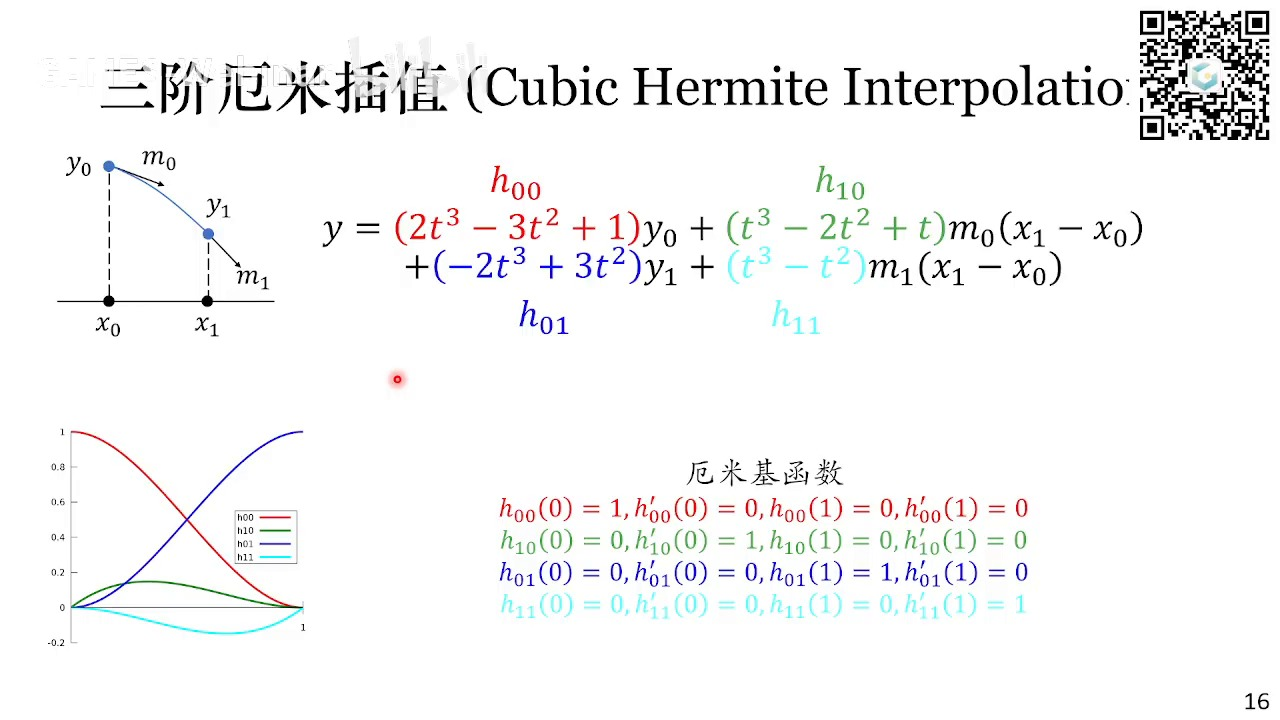
\includegraphics[width=0.92\textwidth]{figures/fig_14_hermite_basis.jpg}
\caption{厄米基函数 $h_{00},h_{10},h_{01},h_{11}$ 及其端点条件\vtag}
\end{figure}
\srcnote{00:33:00--00:33:15}
\end{minipage}


\subsection{如何选择导数}

厄米插值的关键在于：每个采样点上的导数 $m_i$ 是我们自己规定的，只要相邻两段在同一点使用同一个 $m_i$，曲线自然一阶导数连续。常见的选择有：
\[
\begin{gathered}
\text{有限差分：}\ m_i=\frac12\Big(\frac{y_{i+1}-y_i}{x_{i+1}-x_i}+\frac{y_i-y_{i-1}}{x_i-x_{i-1}}\Big),\qquad
\text{Cardinal 样条：}\ m_i=(1-c)\frac{y_{i+1}-y_{i-1}}{x_{i+1}-x_{i-1}},\\
\text{Catmull–Rom 样条（$x_i$ 均匀划分）：}\ m_i=\frac{y_{i+1}-y_{i-1}}{2}.
\end{gathered}
\]
不同的规定方法给出不同的曲线，但都只依赖相邻的点，所以每个点只影响它附近的两段曲线，局部性很好。

\noindent\begin{minipage}{\textwidth}
\begin{figure}[H]
\centering
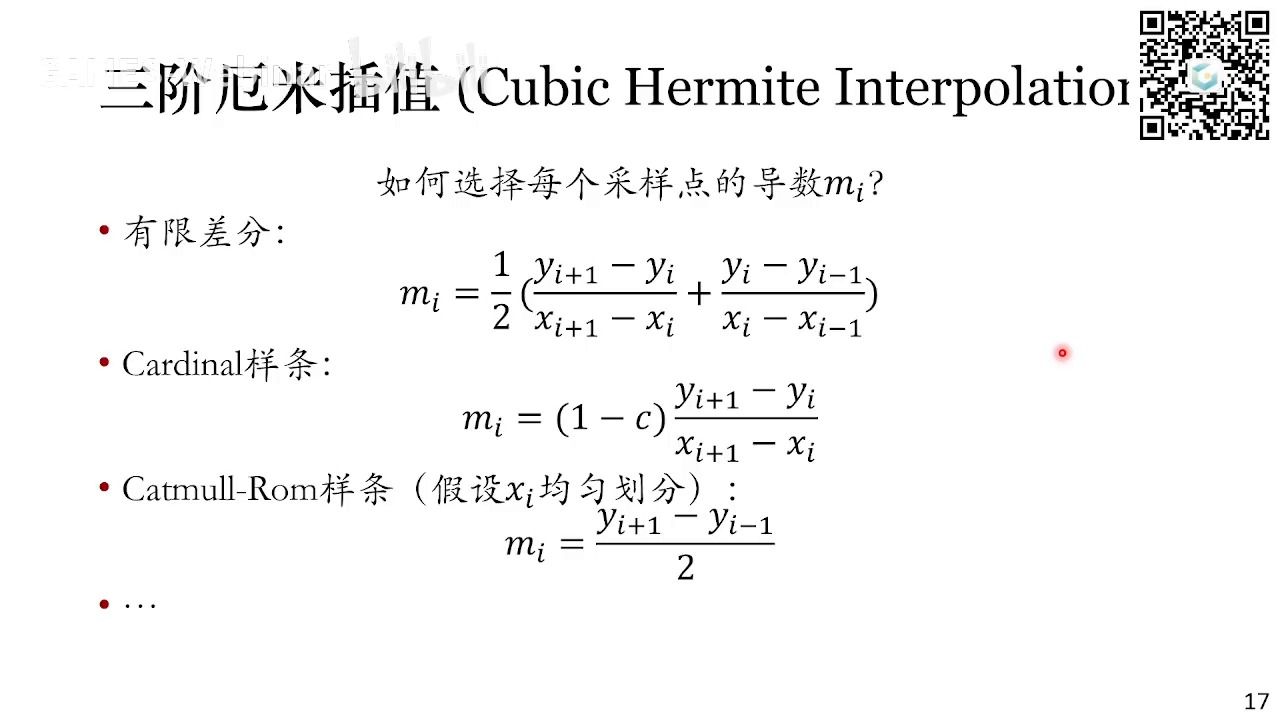
\includegraphics[width=0.92\textwidth]{figures/fig_15_hermite_tangents.jpg}
\caption{如何选择每个采样点的导数：有限差分、Cardinal 样条、Catmull–Rom 样条\vtag}
\end{figure}
\srcnote{00:34:30--00:34:45}
\end{minipage}


\begin{warningbox}{课件中 Cardinal 样条的写法}
讲义作者提醒：课件中 Cardinal 样条写作 $m_i=(1-c)\frac{y_{i+1}-y_i}{x_{i+1}-x_i}$，常见定义为 $m_i=(1-c)\frac{y_{i+1}-y_{i-1}}{x_{i+1}-x_{i-1}}$，其中 $c\in[0,1]$ 是张力参数。$c=0$ 且等距时退化为 Catmull–Rom 样条（导数按 $x$ 归一化后）。上文已按常见定义书写。
\end{warningbox}

\subsection{单调三阶插值}

有些数据本身是单调的，比如累积量、颜色映射表，一般的三阶厄米插值可能在区间内出现“过冲”，破坏单调性。单调三阶插值（monotone cubic interpolation），也称 PCHIP（piecewise cubic Hermite interpolating polynomial），通过调整每个顶点的导数 $m_i$，使插值结果 $C^1$ 连续，并且在每个区间内单调。课件中蓝线是单调插值的结果，红线是一般三阶厄米插值的结果。具体的调整方法见 Fritsch 和 Butland 1984 年发表在 SIAM J. Sci. Comput. 上的论文。

\noindent\begin{minipage}{\textwidth}
\begin{figure}[H]
\centering
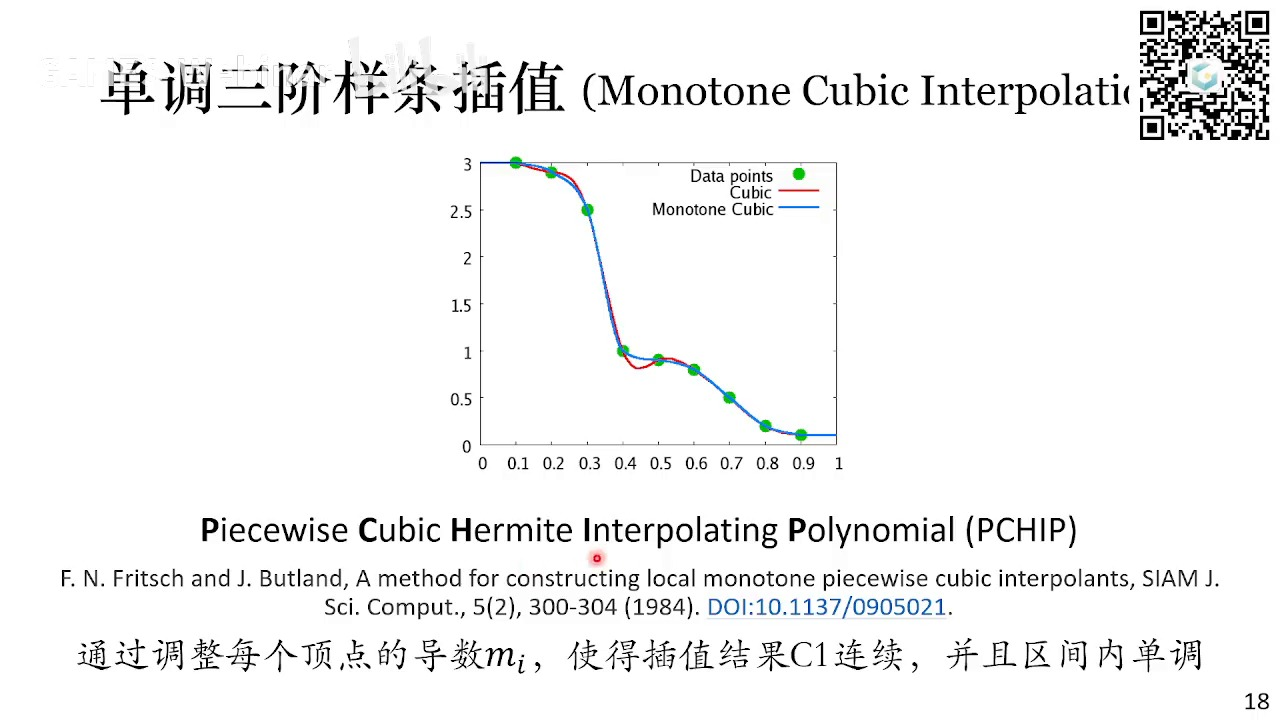
\includegraphics[width=0.92\textwidth]{figures/fig_16_monotone.jpg}
\caption{单调三阶插值（PCHIP）：调整导数使结果在区间内单调\vtag}
\end{figure}
\srcnote{00:36:00--00:36:15}
\end{minipage}


\subsection{插值方法小结}

\begin{itemize}
\item \textbf{线性插值}：$C^0$；计算简单；局部性好。
\item \textbf{多项式插值}：$C^n$，取决于点的个数；有显式公式；局部性差，且有龙格现象。
\item \textbf{二阶样条}：$C^1$；需要解方程；局部性差。
\item \textbf{三阶样条}：$C^2$；需要解方程；局部性差。
\item \textbf{三阶厄米插值}：$C^1$；计算简单；局部性好。
\item \textbf{单调三阶插值}：$C^1$；计算简单；局部性好，且保持单调。
\end{itemize}

讲者总结说，二阶、三阶样条和多项式插值的局部性都不好，三阶厄米插值则在连续性、复杂性和局部性之间取得了很好的平衡，所以应用最广泛。

\noindent\begin{minipage}{\textwidth}
\begin{figure}[H]
\centering
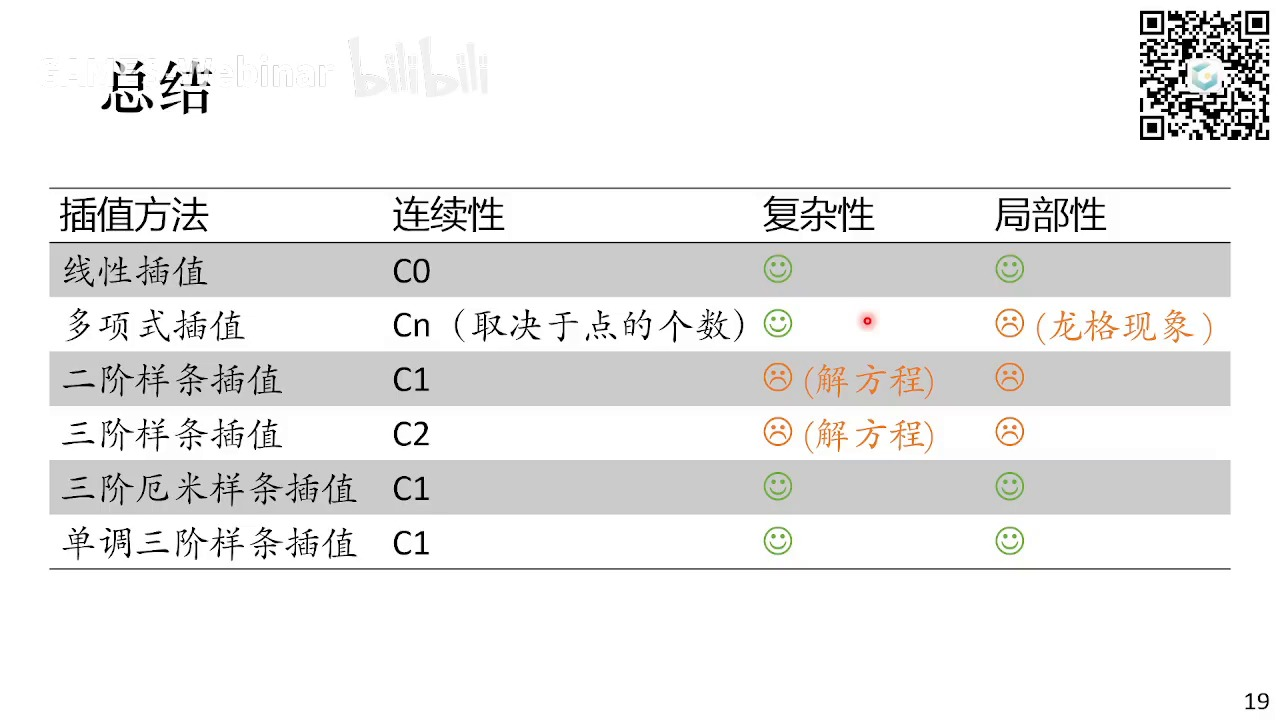
\includegraphics[width=0.92\textwidth]{figures/fig_17_interp_summary.jpg}
\caption{插值方法总结：连续性、复杂性与局部性\vtag}
\end{figure}
\srcnote{00:38:00--00:38:15}
\end{minipage}


\section{基函数的视角}

\subsection{线性插值的基函数}

接下来讲者引入一个非常重要的概念：\textbf{基函数}（basis function）。它的形状像一顶“帽子”：
\[
B_i(x)=\begin{cases}\dfrac{x-x_{i-1}}{x_i-x_{i-1}},&x\in[x_{i-1},x_i]\\[2mm]\dfrac{x_{i+1}-x}{x_{i+1}-x_i},&x\in[x_i,x_{i+1}]\\[2mm]0,&\text{else}\end{cases}
\qquad B_i(x_j)=\delta_{ij}.
\]
在区间 $[x_i,x_{i+1}]$ 上，$B_i$ 从一线性降到零，$B_{i+1}$ 从零线性升到一，于是线性插值可以写成 $y=B_i(x)y_i+B_{i+1}(x)y_{i+1}$，对整个定义域就是
\[
y(x)=\sum_iy_iB_i(x).
\]

\noindent\begin{minipage}{\textwidth}
\begin{figure}[H]
\centering
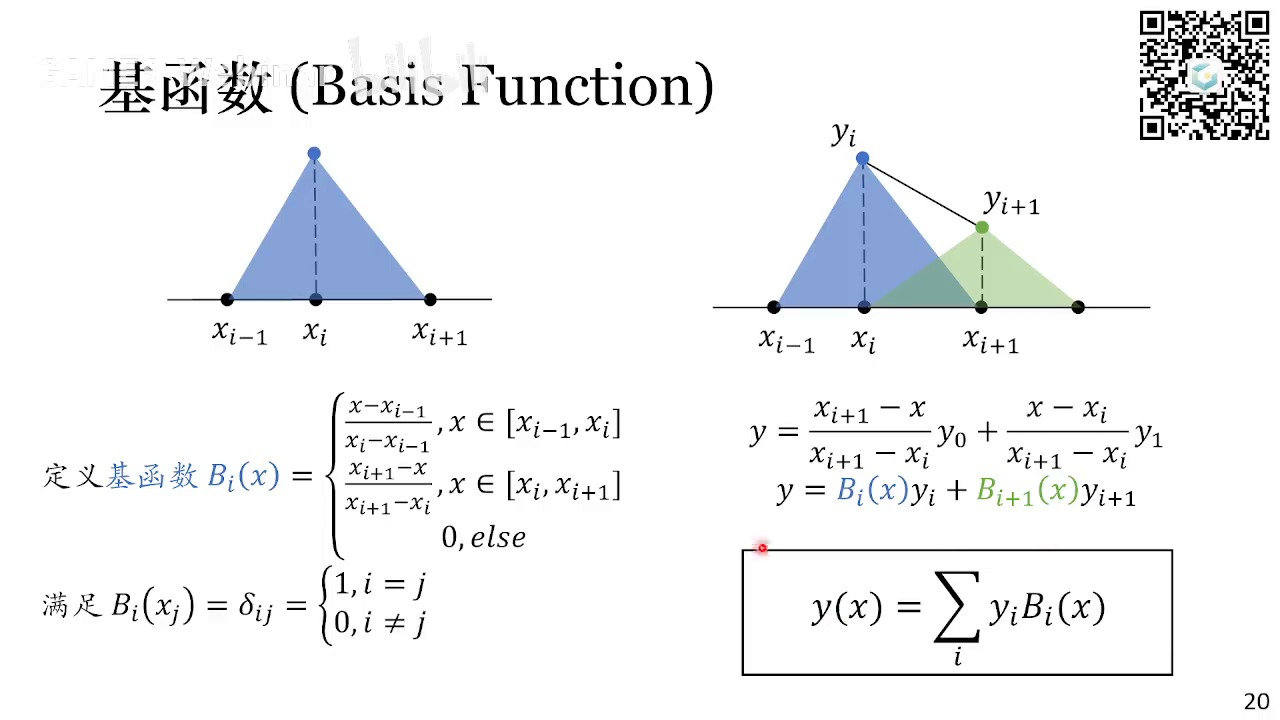
\includegraphics[width=0.92\textwidth]{figures/fig_18_basis_linear.jpg}
\caption{线性插值的基函数：“帽子”函数 $B_i$\vtag}
\end{figure}
\srcnote{00:41:00--00:41:15}
\end{minipage}


\subsection{基函数统一了插值}

讲者说，大部分插值方法都可以理解成 $y(x)=\sum_iy_iB_i(x)$ 的形式，唯一的不同是每种方法得到的基函数不同。这个视角带来三点好处：它为插值提供了新的观察视角；可以通过改变基函数来定义新的插值方式；只要满足 $B_i(x_j)=\delta_{ij}$，就能保证插值结果经过采样点：
\[
y(x_i)=\sum_jy_jB_j(x_i)=\sum_jy_j\delta_{ij}=y_i .
\]

\noindent\begin{minipage}{\textwidth}
\begin{figure}[H]
\centering
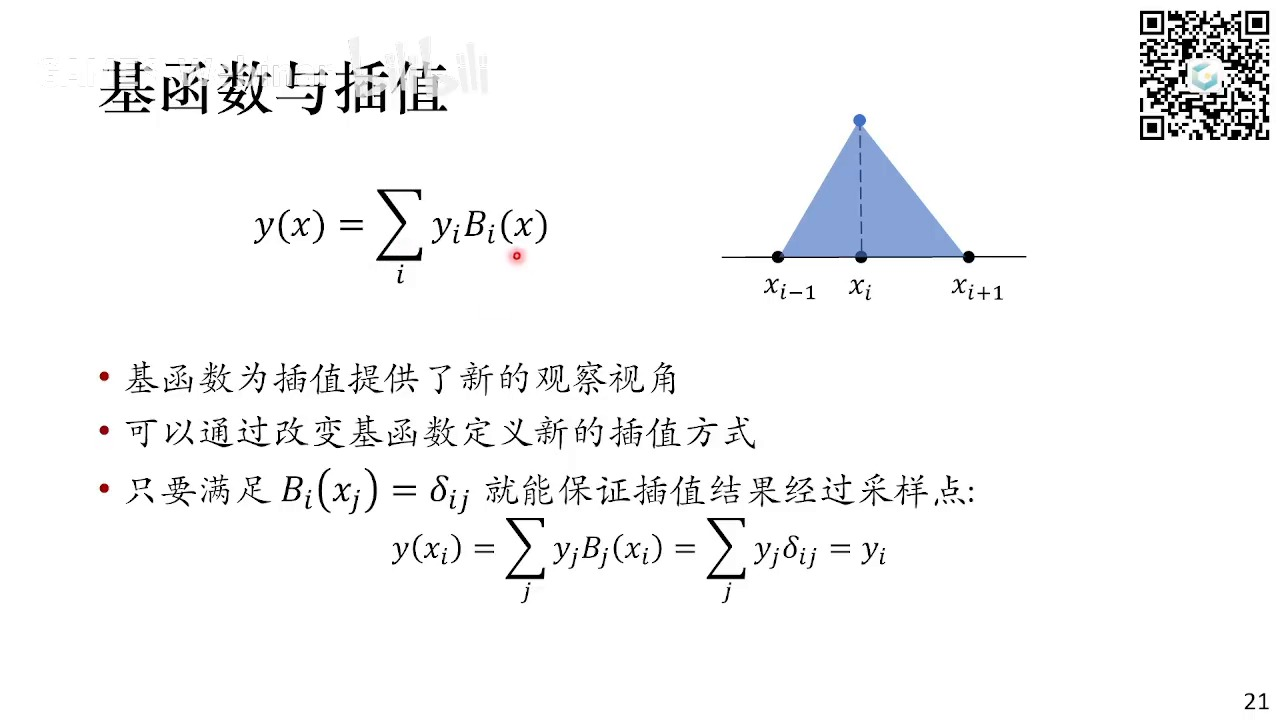
\includegraphics[width=0.92\textwidth]{figures/fig_19_basis_interp.jpg}
\caption{基函数与插值：只要 $B_i(x_j)=\delta_{ij}$ 就满足插值条件\vtag}
\end{figure}
\srcnote{00:42:30--00:42:45}
\end{minipage}


把各种插值方法的基函数画出来比较：多项式插值的基函数就是拉格朗日多项式，课件中 4 个点对应 4 个三次多项式，每一个都在整个区间上起伏；三阶样条的基函数需要通过求解方程得到，同样遍布整个区间；三阶厄米样条的基函数则只在采样点附近非零，具有局部性，并且当 $x_i$ 间隔相同时，所有 $B_i$ 的形状都相同，只是平移了一下。讲者说，这个“形状相同、只做平移”的性质会在很多事情上对我们有帮助，比如后面的卷积和采样理论。

\begin{knowledgebox}{平移不变的基函数}
讲义作者补充：当所有基函数都是同一个函数 $B$ 的平移，$B_i(x)=B(x-x_i)$，插值就可以写成 $y(x)=\sum_iy_iB(x-x_i)$，这正是离散采样序列与核函数 $B$ 的卷积。线性插值对应“帽子”核，厄米插值对应三次核。下一讲的傅里叶变换会告诉我们，不同核在频域中保留和抑制了哪些频率，从而从另一个角度解释各种插值方法的效果差异。
\end{knowledgebox}

\noindent\begin{minipage}{\textwidth}
\begin{figure}[H]
\centering
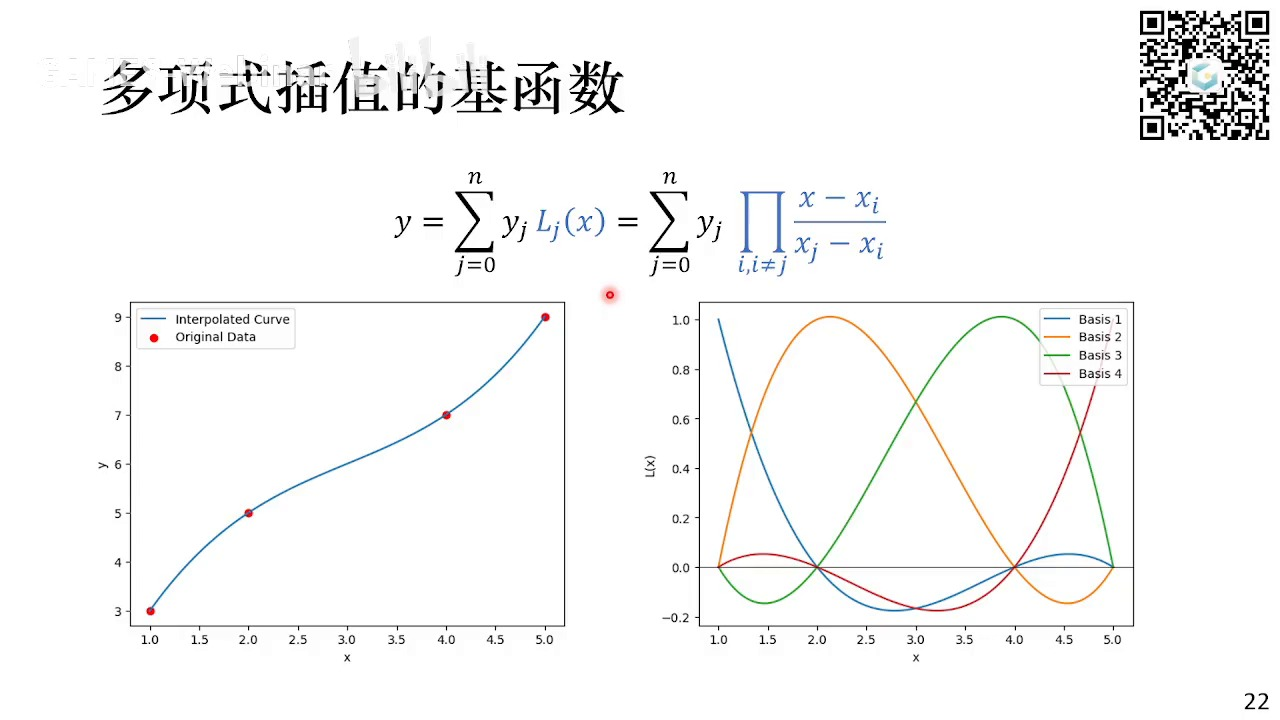
\includegraphics[width=0.92\textwidth]{figures/fig_20_basis_poly.jpg}
\caption{多项式插值的基函数：拉格朗日多项式遍布整个区间\vtag}
\end{figure}
\srcnote{00:44:15--00:44:30}
\end{minipage}


\noindent\begin{minipage}{\textwidth}
\begin{figure}[H]
\centering
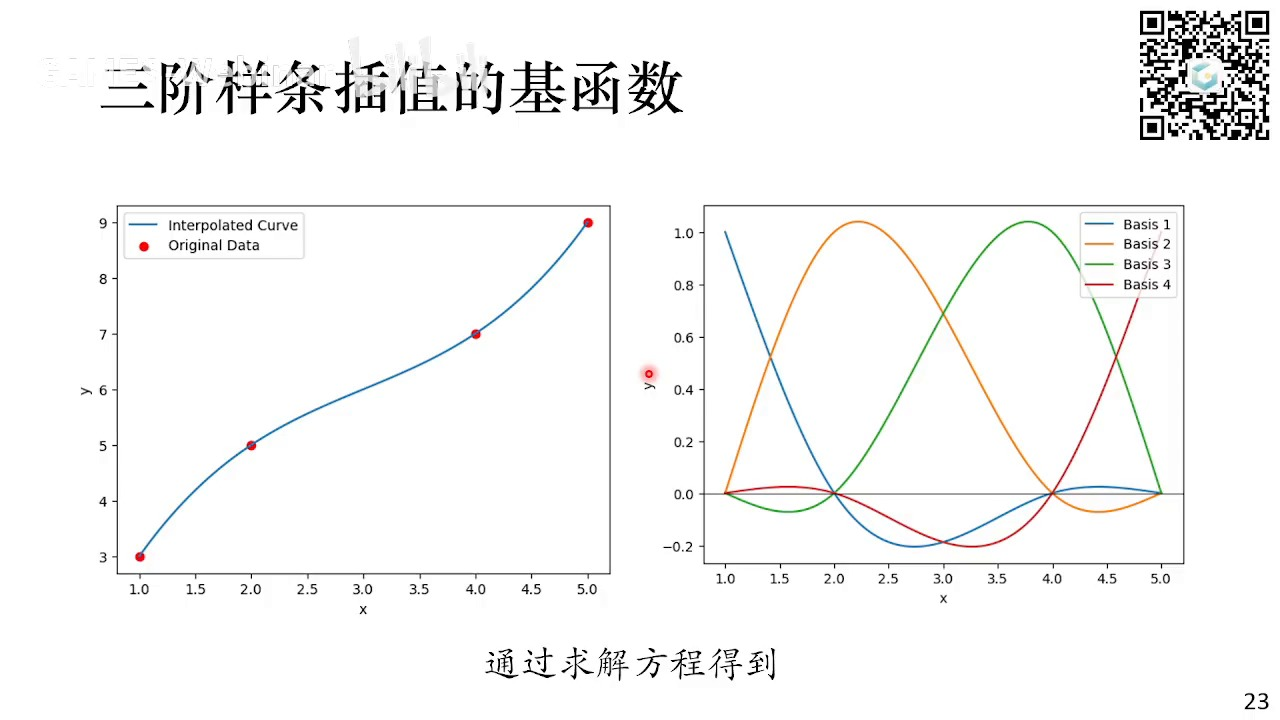
\includegraphics[width=0.92\textwidth]{figures/fig_21_basis_cubic.jpg}
\caption{三阶样条插值的基函数：通过求解方程得到，同样是全局的\vtag}
\end{figure}
\srcnote{00:45:00--00:45:15}
\end{minipage}


\noindent\begin{minipage}{\textwidth}
\begin{figure}[H]
\centering
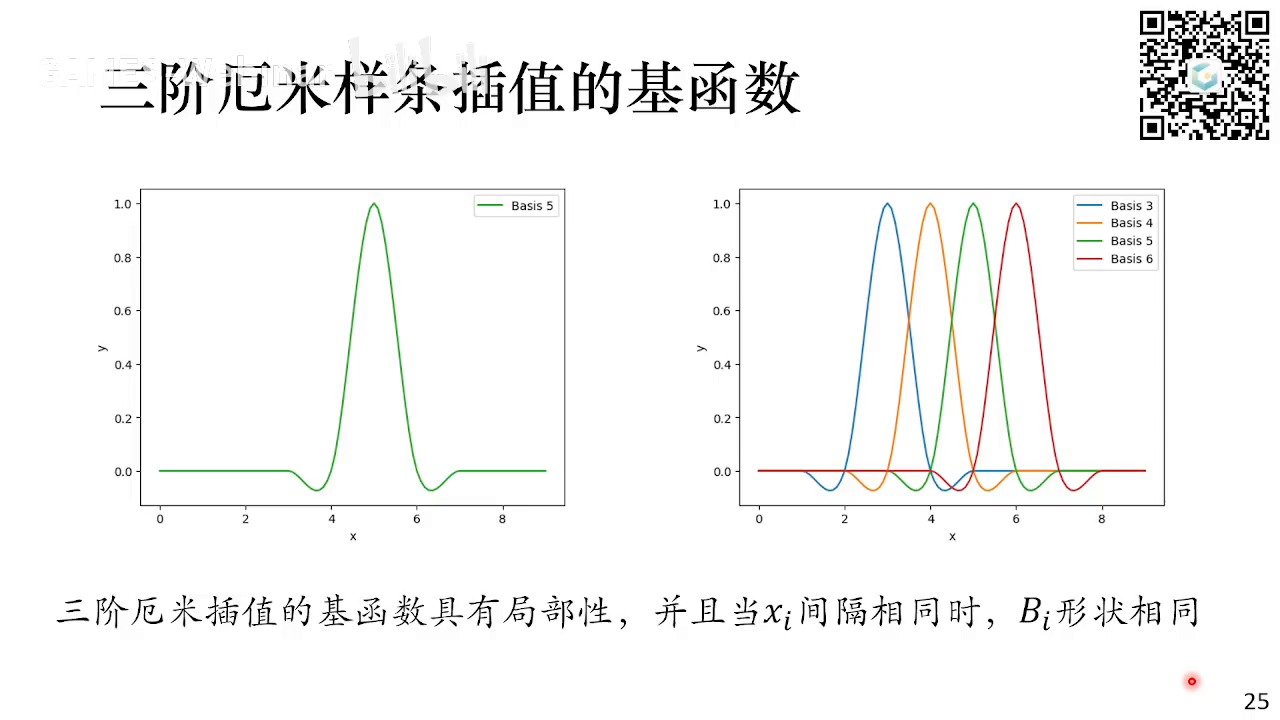
\includegraphics[width=0.92\textwidth]{figures/fig_22_basis_hermite.jpg}
\caption{三阶厄米样条插值的基函数：局部支撑，等距时形状相同\vtag}
\end{figure}
\srcnote{00:48:00--00:48:15}
\end{minipage}


讲者推荐了 Freya Holmér 在 YouTube 上关于样条的视频（B 站也有搬运），认为讲得非常好，对厄米样条感兴趣的同学可以仔细看一看。

\section{高维插值}

前面介绍的都是一维插值。高维中常见的插值问题包括曲线插值、多边形插值、像素插值和点云插值。

\noindent\begin{minipage}{\textwidth}
\begin{figure}[H]
\centering
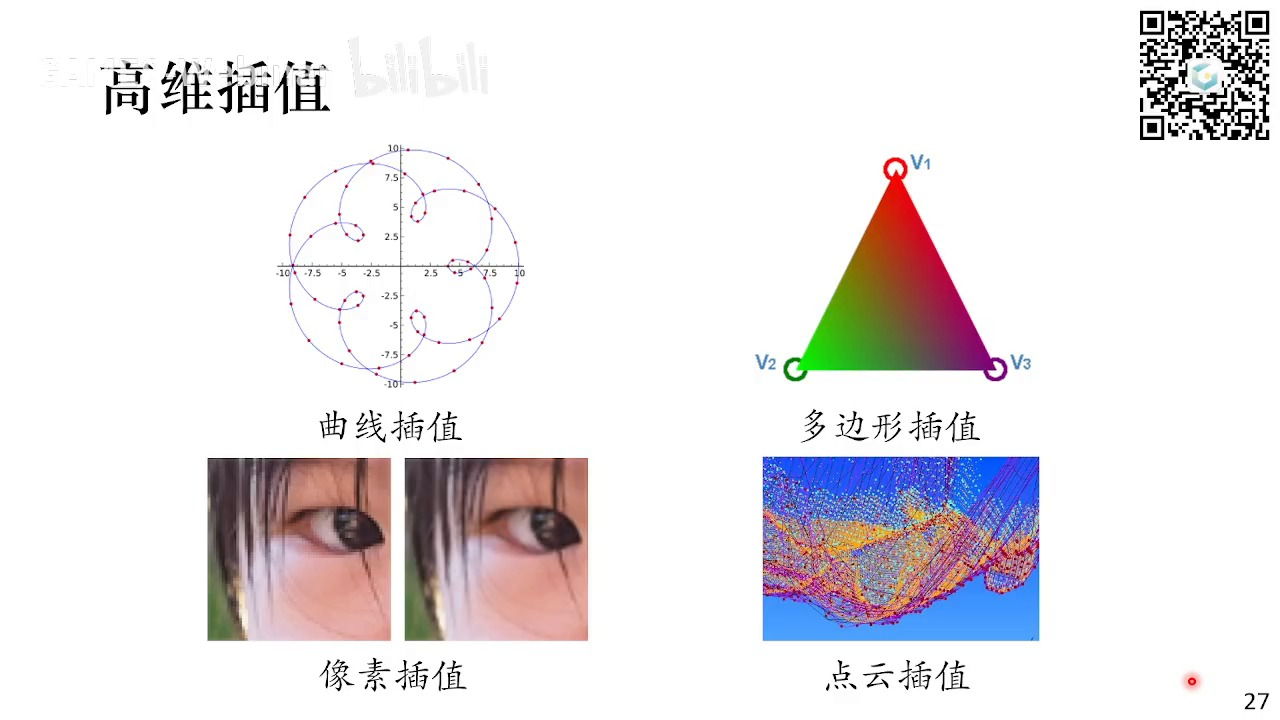
\includegraphics[width=0.92\textwidth]{figures/fig_23_high_dim.jpg}
\caption{高维插值：曲线、多边形、像素与点云\vtag}
\end{figure}
\srcnote{00:49:45--00:50:00}
\end{minipage}


\subsection{曲线插值}

曲线插值的问题是：空间中按顺序给定一系列点 $\mathbf p_0,\dots,\mathbf p_n$，插值出中间的曲线 $\mathbf p(t)$，可以认为在相邻点之间 $t\in[0,1]$。直接推广三阶厄米插值，把原来的标量 $y_0,y_1$ 换成点，把导数换成切向量，就得到
\[
\mathbf p(t)=(2t^3-3t^2+1)\mathbf p_0+(t^3-2t^2+t)\mathbf m_0+(-2t^3+3t^2)\mathbf p_1+(t^3-t^2)\mathbf m_1 .
\]
它经过所有控制点。讲者提到，PowerPoint 里的曲线工具用的就是这种三阶厄米样条曲线。

\noindent\begin{minipage}{\textwidth}
\begin{figure}[H]
\centering
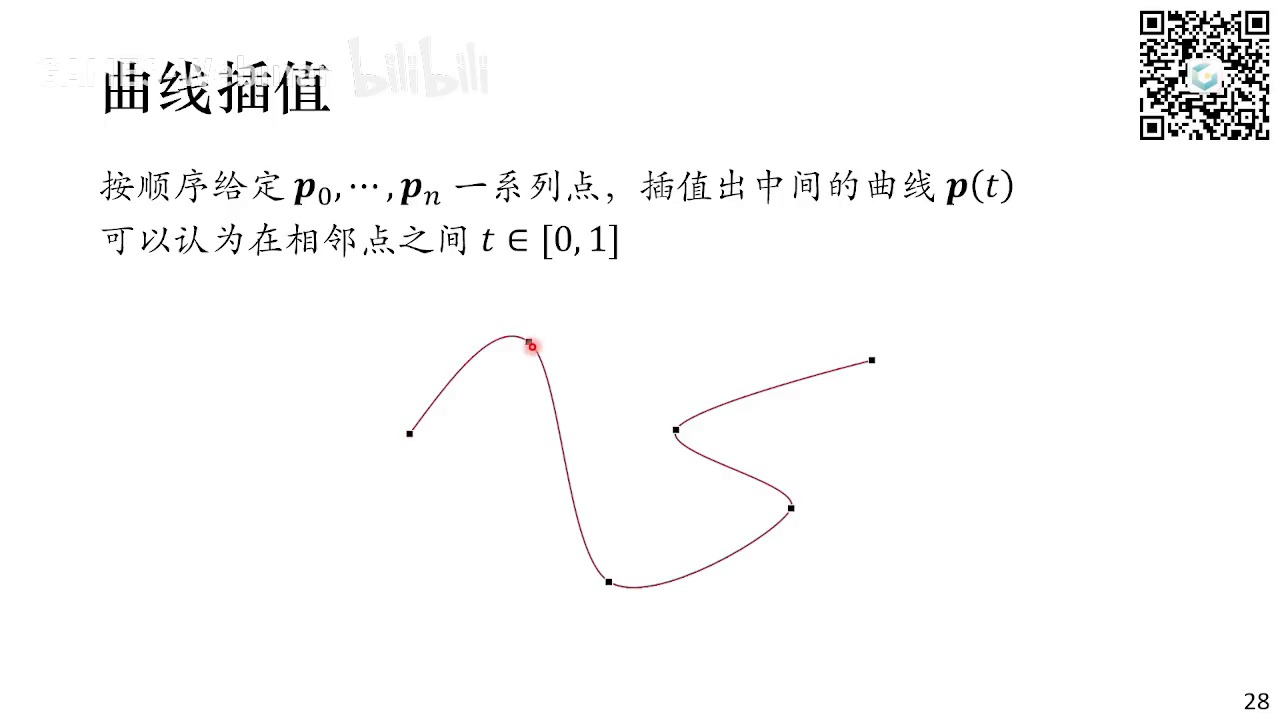
\includegraphics[width=0.92\textwidth]{figures/fig_24_curve_interp.jpg}
\caption{曲线插值：按顺序给定点，插值出中间的曲线\vtag}
\end{figure}
\srcnote{00:50:45--00:51:00}
\end{minipage}


\noindent\begin{minipage}{\textwidth}
\begin{figure}[H]
\centering
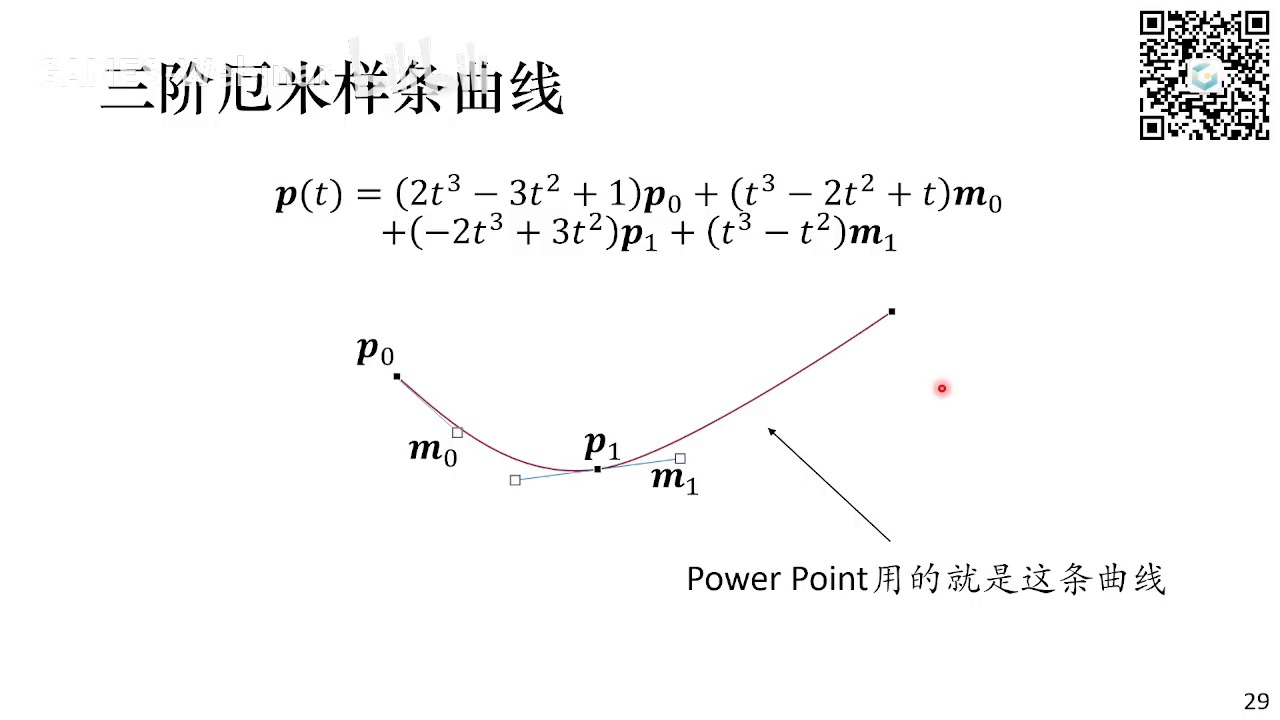
\includegraphics[width=0.92\textwidth]{figures/fig_25_hermite_curve.jpg}
\caption{三阶厄米样条曲线：PowerPoint 的曲线工具就是这条曲线\vtag}
\end{figure}
\srcnote{00:52:15--00:52:30}
\end{minipage}


\begin{knowledgebox}{插值曲线与一般曲线}
图形学中的曲线并不一定要经过控制点。经过所有控制点的曲线称为插值曲线（interpolation curve）。最常用的贝塞尔曲线（Bézier curve）和 B 样条曲线（B-spline curve）都不经过（全部）控制点，因此不是插值曲线，它们更接近“拟合”的思路。关于曲线的更多知识可以学习 GAMES102。
\end{knowledgebox}

\noindent\begin{minipage}{\textwidth}
\begin{figure}[H]
\centering
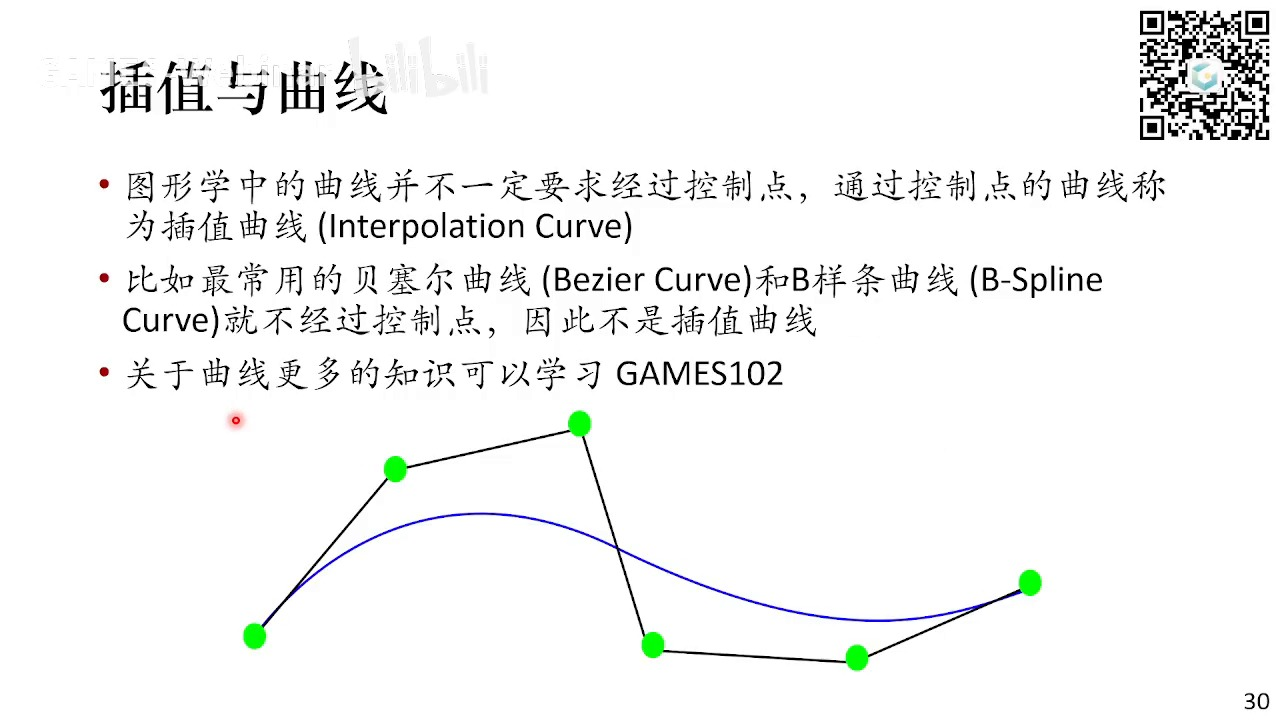
\includegraphics[width=0.92\textwidth]{figures/fig_26_curves.jpg}
\caption{插值曲线与贝塞尔、B 样条曲线\vtag}
\end{figure}
\srcnote{00:53:30--00:53:45}
\end{minipage}


\subsection{三角形与多边形插值}

三角形内的插值用\textbf{重心坐标}（barycentric interpolation）。对三角形 $ABC$ 内一点 $P$，权重 $\alpha$ 定义为 $P$ 与 $A$ 对边构成的三角形面积除以总面积，$\beta$、$\gamma$ 同理，满足 $\alpha+\beta+\gamma=1$，插值结果为 $f(P)=\alpha f_A+\beta f_B+\gamma f_C$。把重心坐标当作基函数画出来，它也是“帽子”形状：在对应顶点取一，在另外两个顶点取零。这与一维线性插值的基函数完全类似。GAMES101 的插值与纹理映射一讲中有详细介绍。

\noindent\begin{minipage}{\textwidth}
\begin{figure}[H]
\centering
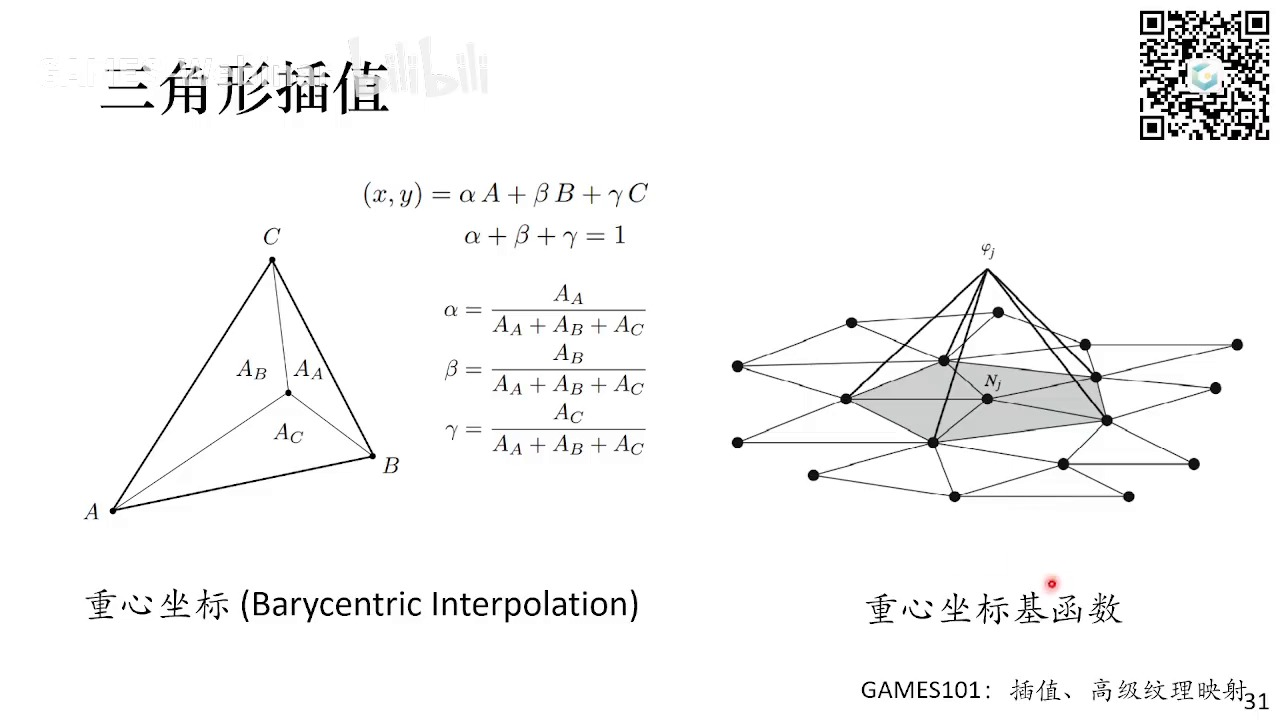
\includegraphics[width=0.92\textwidth]{figures/fig_27_barycentric.jpg}
\caption{三角形插值：重心坐标及其基函数\vtag}
\end{figure}
\srcnote{00:56:30--00:56:45}
\end{minipage}


对一般多边形，可以用\textbf{均值坐标}（mean value coordinates）。它的权重分布同样满足：在对应顶点取一，向其它顶点逐渐减小。

\noindent\begin{minipage}{\textwidth}
\begin{figure}[H]
\centering
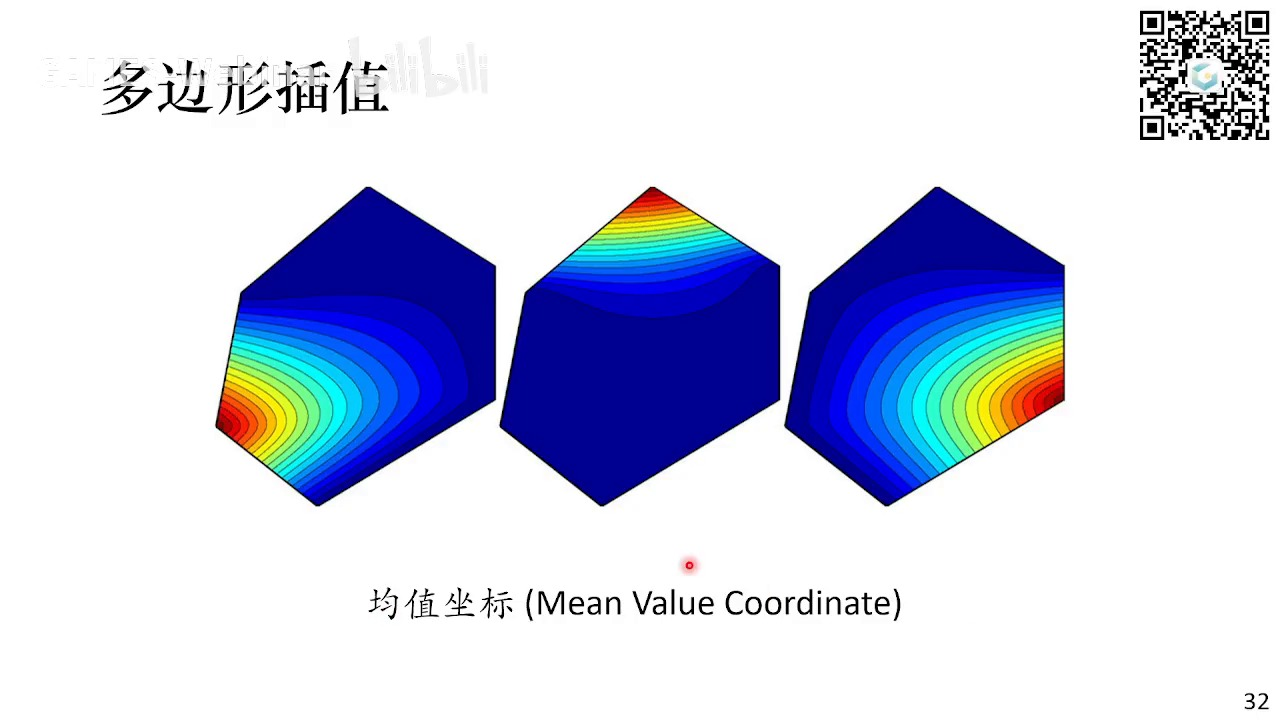
\includegraphics[width=0.92\textwidth]{figures/fig_28_mean_value.jpg}
\caption{多边形插值：均值坐标的权重分布\vtag}
\end{figure}
\srcnote{00:57:30--00:57:45}
\end{minipage}


\subsection{像素插值}

图像缩放时需要在像素之间插值。一维的最近邻、线性和三次插值，推广到二维像素网格上，就是最近邻（nearest）、双线性（bilinear）和双三次（bicubic）插值：沿 $x$、$y$ 方向分别做一维插值。双三次插值通常就是双三次厄米插值。放大一张眼睛的图片对比，最近邻有明显的马赛克，双线性比较模糊，双三次最清晰。

\noindent\begin{minipage}{\textwidth}
\begin{figure}[H]
\centering
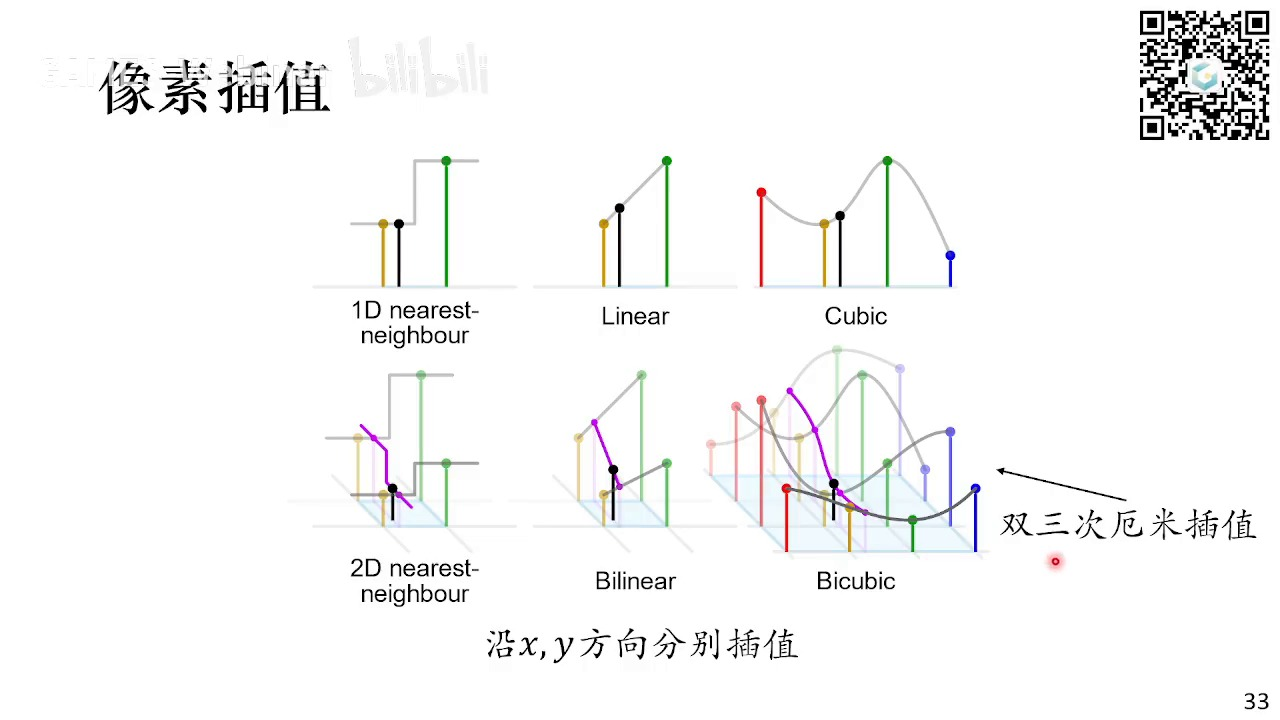
\includegraphics[width=0.92\textwidth]{figures/fig_29_pixel_interp.jpg}
\caption{像素插值：沿 $x,y$ 方向分别插值，得到双线性、双三次插值\vtag}
\end{figure}
\srcnote{00:58:30--00:58:45}
\end{minipage}


\noindent\begin{minipage}{\textwidth}
\begin{figure}[H]
\centering
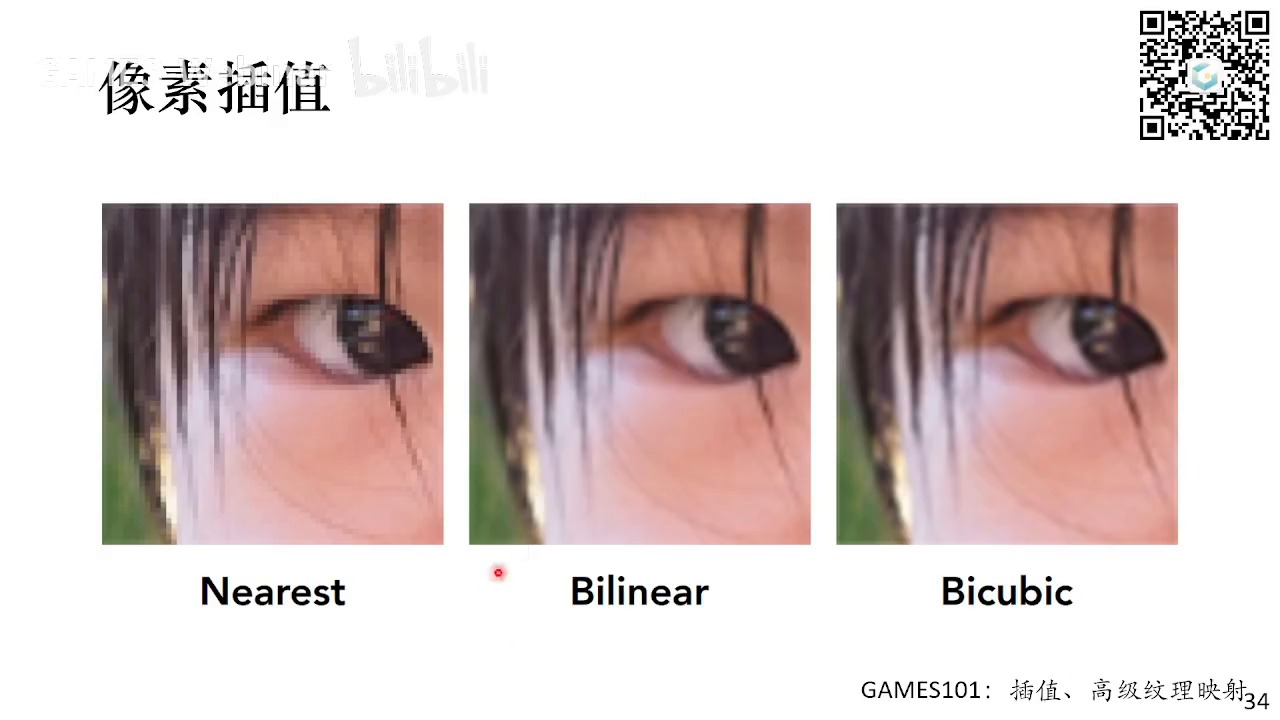
\includegraphics[width=0.92\textwidth]{figures/fig_30_pixel_compare.jpg}
\caption{最近邻、双线性与双三次插值的效果对比\vtag}
\end{figure}
\srcnote{00:59:00--00:59:15}
\end{minipage}


\subsection{点云插值与径向基函数}

点云插值的问题是：空间中有一堆散乱的采样点 $\mathbf x_i$，每个点上有一个函数值，可以是颜色、法向等等，如何插值出任意位置的值？常用\textbf{径向基函数}（radial basis function, RBF），也叫核函数（kernel function）$\varphi(\|\mathbf x-\mathbf x_i\|)$。它只与到采样点的距离有关，因此是对称的。常见的核函数有
\[
\text{高斯核：}\ \exp(-(\varepsilon r)^2),\qquad
\text{拉普拉斯核：}\ \exp(-\varepsilon r),\qquad
\text{二次有理核：}\ \frac{1}{1+(\varepsilon r)^2}.
\]

\noindent\begin{minipage}{\textwidth}
\begin{figure}[H]
\centering
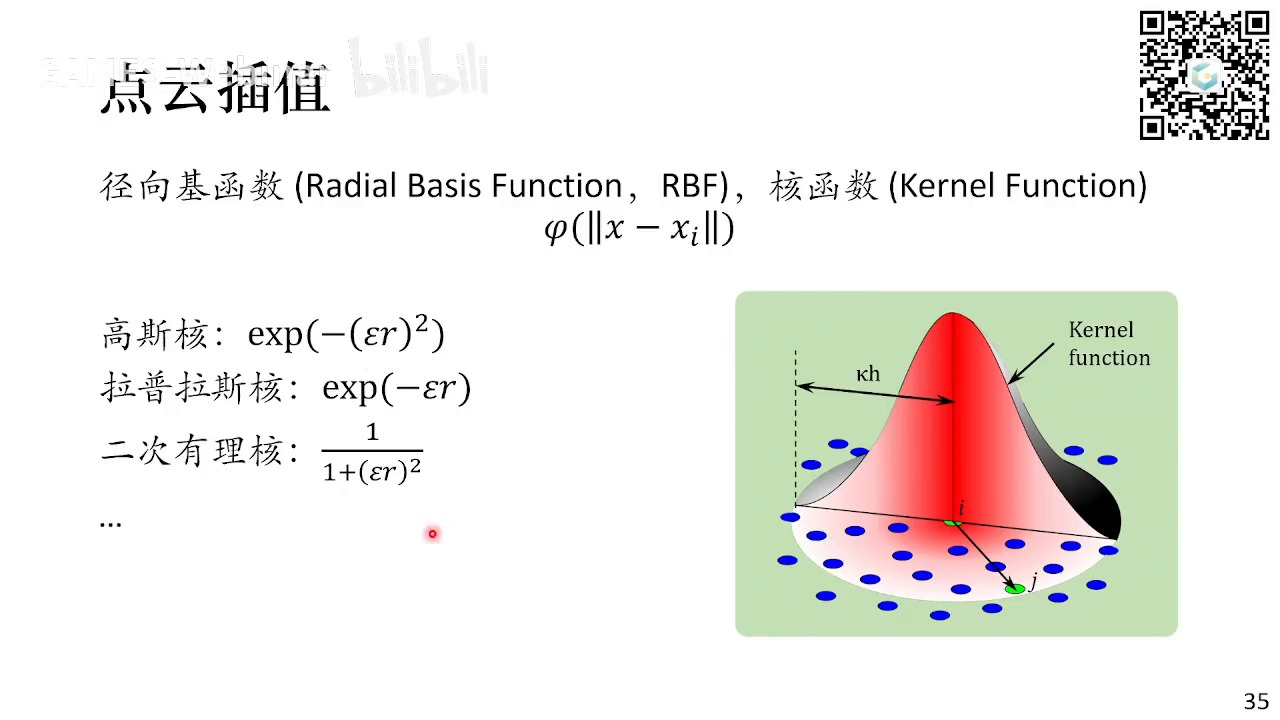
\includegraphics[width=0.92\textwidth]{figures/fig_31_rbf.jpg}
\caption{径向基函数：只与距离有关的对称核函数\vtag}
\end{figure}
\srcnote{01:00:30--01:00:45}
\end{minipage}


插值函数写成核函数的加权和 $f(\mathbf x)=\sum_iy_i\varphi(\|\mathbf x-\mathbf x_i\|)$。权重 $y_i$ 是未知的，由插值条件 $f(\mathbf x_i)=f_i$ 确定，$n$ 个采样点给出 $n$ 个方程：
\[
\begin{pmatrix}\varphi(\|\mathbf x_0-\mathbf x_0\|)&\cdots&\varphi(\|\mathbf x_0-\mathbf x_{n-1}\|)\\ \vdots&\ddots&\vdots\\ \varphi(\|\mathbf x_{n-1}-\mathbf x_0\|)&\cdots&\varphi(\|\mathbf x_{n-1}-\mathbf x_{n-1}\|)\end{pmatrix}
\begin{pmatrix}y_0\\ \vdots\\ y_{n-1}\end{pmatrix}=
\begin{pmatrix}f_0\\ \vdots\\ f_{n-1}\end{pmatrix}.
\]
这是 $n\times n$ 的对称矩阵方程，$n$ 为点的个数。解出 $y_i$ 后，就能求任意位置的值。

\noindent\begin{minipage}{\textwidth}
\begin{figure}[H]
\centering
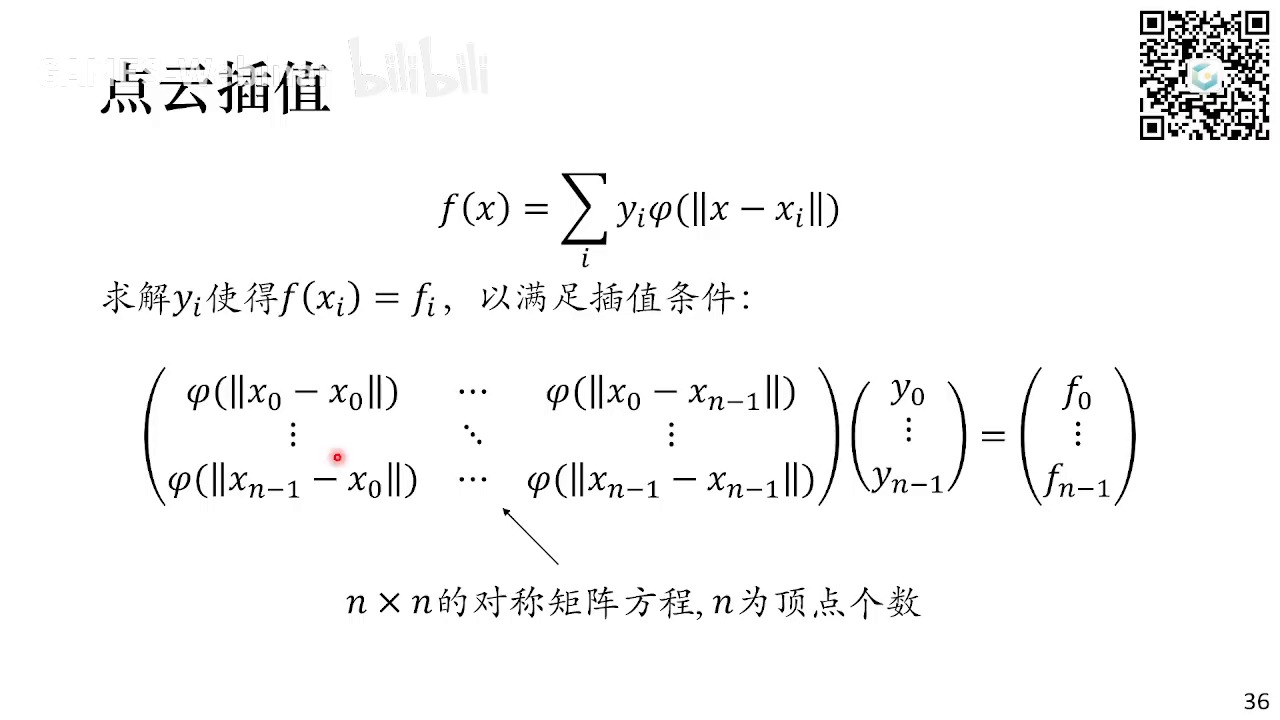
\includegraphics[width=0.92\textwidth]{figures/fig_32_rbf_solve.jpg}
\caption{点云插值：由插值条件得到 $n\times n$ 对称矩阵方程\vtag}
\end{figure}
\srcnote{01:02:15--01:02:30}
\end{minipage}


\noindent\begin{minipage}{\textwidth}
\begin{figure}[H]
\centering
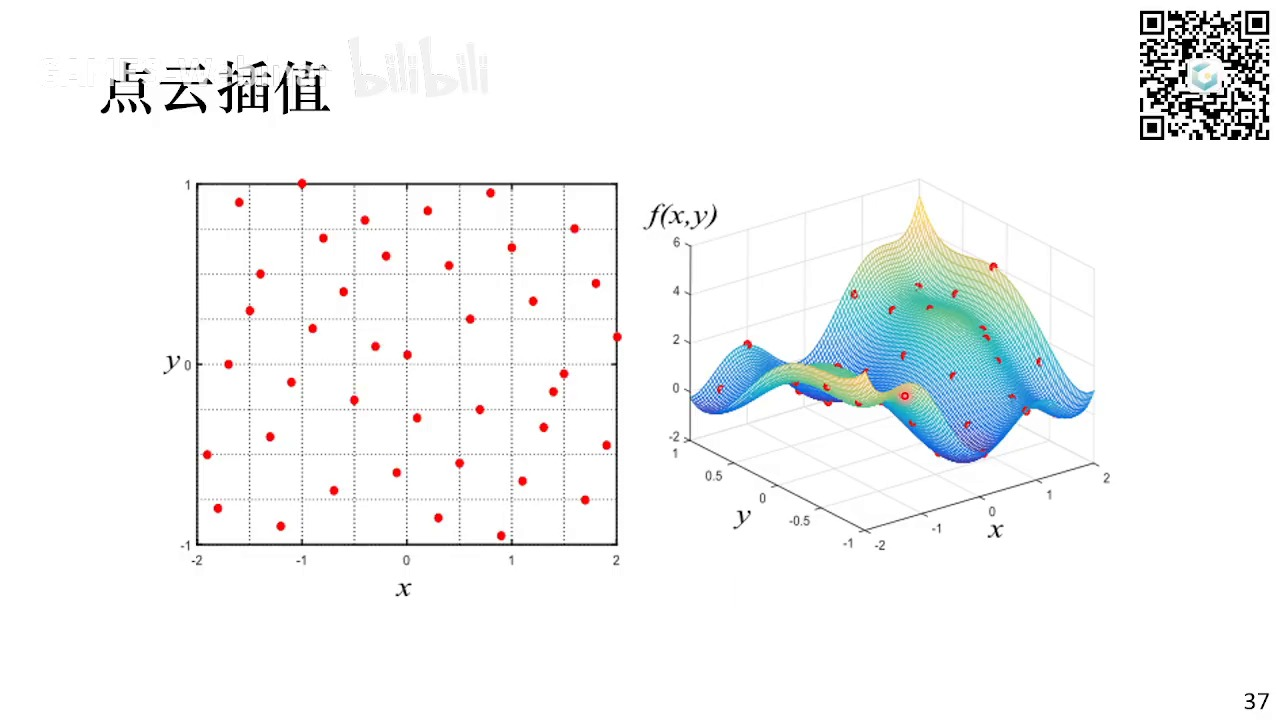
\includegraphics[width=0.92\textwidth]{figures/fig_33_rbf_result.jpg}
\caption{点云插值的结果：散乱点上的值插值成光滑曲面\vtag}
\end{figure}
\srcnote{01:03:00--01:03:15}
\end{minipage}


\subsection{用点云表达连续场}

讲者指出，比起在点云上严格插值，更常见的情况是用点云\emph{近似表达}一个连续场。此时放弃插值条件 $f(\mathbf x_i)=f_i$，认为每个顶点表达的是空间中由核函数定义的一定范围内的分布，直接给出
\[
f(\mathbf x)=\sum_if_i\,\varphi(\|\mathbf x-\mathbf x_i\|),\qquad \int_\Omega\varphi(\|\mathbf x-\mathbf x_i\|)\,\mathrm dV=1 .
\]
与前面唯一的区别是：系数直接就是 $f_i$，不需要解方程。这时 $f(\mathbf x_i)\neq f_i$，但一般要假定核函数满足归一化条件（讲者在答疑时更正，核函数前要乘一个系数使其积分为一）。归一化后，相当于把每个点上的值“撒”到了整个空间，但整体集中在 $\mathbf x_i$ 附近。SPH 流体和 3D Gaussian Splatting 都是这种做法：在 3DGS 中，核函数是高斯函数，$f_i$ 可以是每个点的颜色、不透明度等。

\noindent\begin{minipage}{\textwidth}
\begin{figure}[H]
\centering
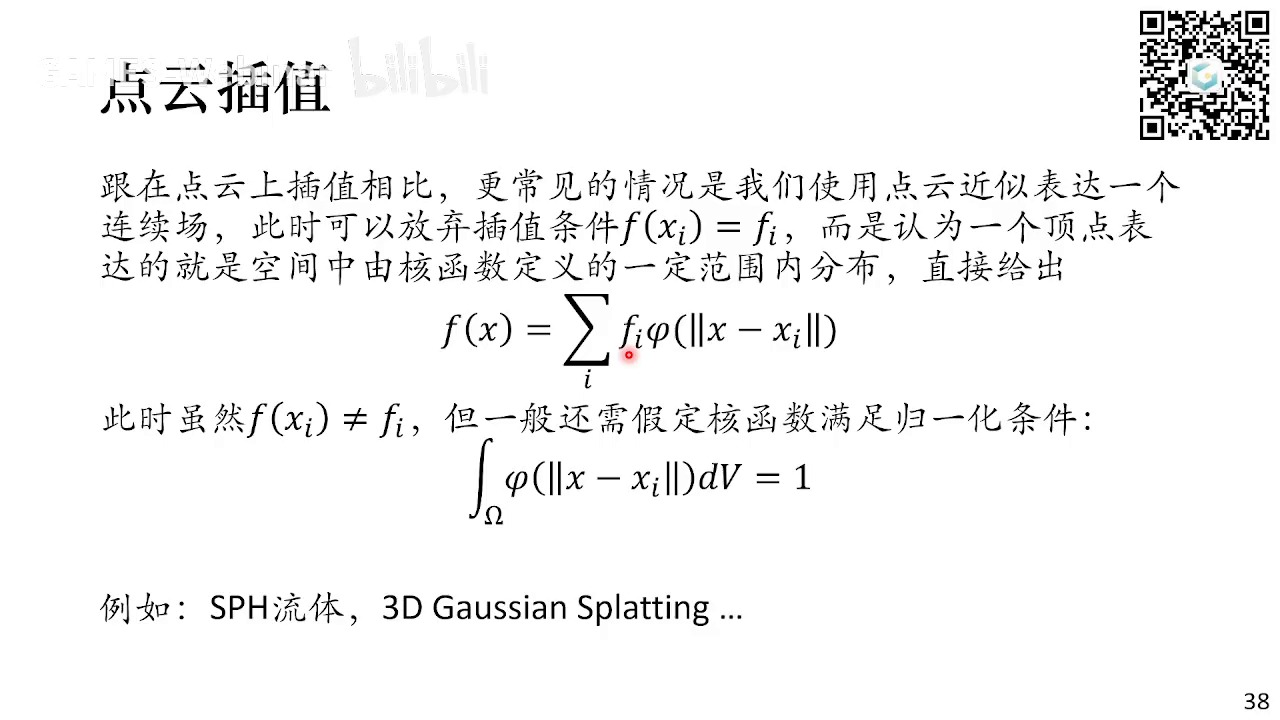
\includegraphics[width=0.92\textwidth]{figures/fig_34_rbf_field.jpg}
\caption{用点云近似表达连续场：放弃插值条件，要求核函数归一化（SPH、3D Gaussian Splatting）\vtag}
\end{figure}
\srcnote{01:06:15--01:06:30}
\end{minipage}


\section{拟合}

\subsection{拟合问题}

拟合假定数据分布满足某种规律 $y=f_\theta(x)$，寻找最佳的参数，使误差最小：
\[
\theta^*=\operatorname*{argmin}_\theta\sum_i\mathrm{Dist}\big(f_\theta(x_i),y_i\big).
\]
讲者说，前一部分“假定规律”是我们对整个分布的先验，后一部分“最小化误差”是优化的过程。

\noindent\begin{minipage}{\textwidth}
\begin{figure}[H]
\centering
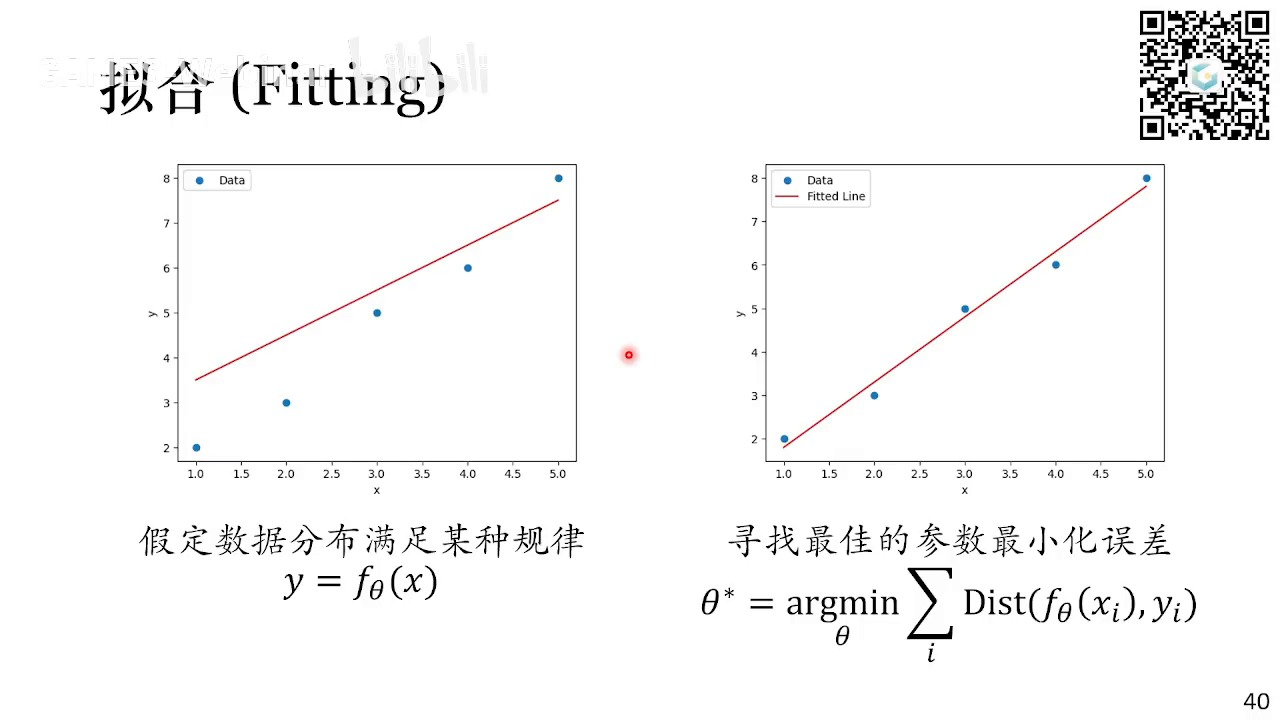
\includegraphics[width=0.92\textwidth]{figures/fig_35_fitting.jpg}
\caption{拟合：假定规律 $y=f_\theta(x)$，寻找最佳参数最小化误差\vtag}
\end{figure}
\srcnote{01:08:00--01:08:15}
\end{minipage}


\subsection{最小二乘法}

大家最熟悉的拟合方法是最小二乘法（least squares）。它假定函数对参数是\emph{线性}的，但对 $x$ 可以是任意函数：
\[
y=a_1x+a_0,\qquad y=a_2x^2+a_1x+a_0,\qquad y=a_1\sqrt x+a_0,\qquad\cdots
\]
统一写成
\[
y=\begin{pmatrix}g_0(x)&\cdots&g_{k-1}(x)\end{pmatrix}\begin{pmatrix}a_0\\ \vdots\\ a_{k-1}\end{pmatrix}=\mathbf g^{\mathsf T}(x)\,\mathbf a ,
\]
其中 $g_j$ 都是已知形式、不含未知数的函数，所有未知数都放在 $\mathbf a$ 里。给定数据集 $(x_0,y_0)$, $\dots$, $(x_{n-1},y_{n-1})$，最小化
\[
\sum_i\big(y_i-\mathbf g^{\mathsf T}(x_i)\mathbf a\big)^2 ,
\]
即图中每一条竖直残差线段的平方和。

\noindent\begin{minipage}{\textwidth}
\begin{figure}[H]
\centering
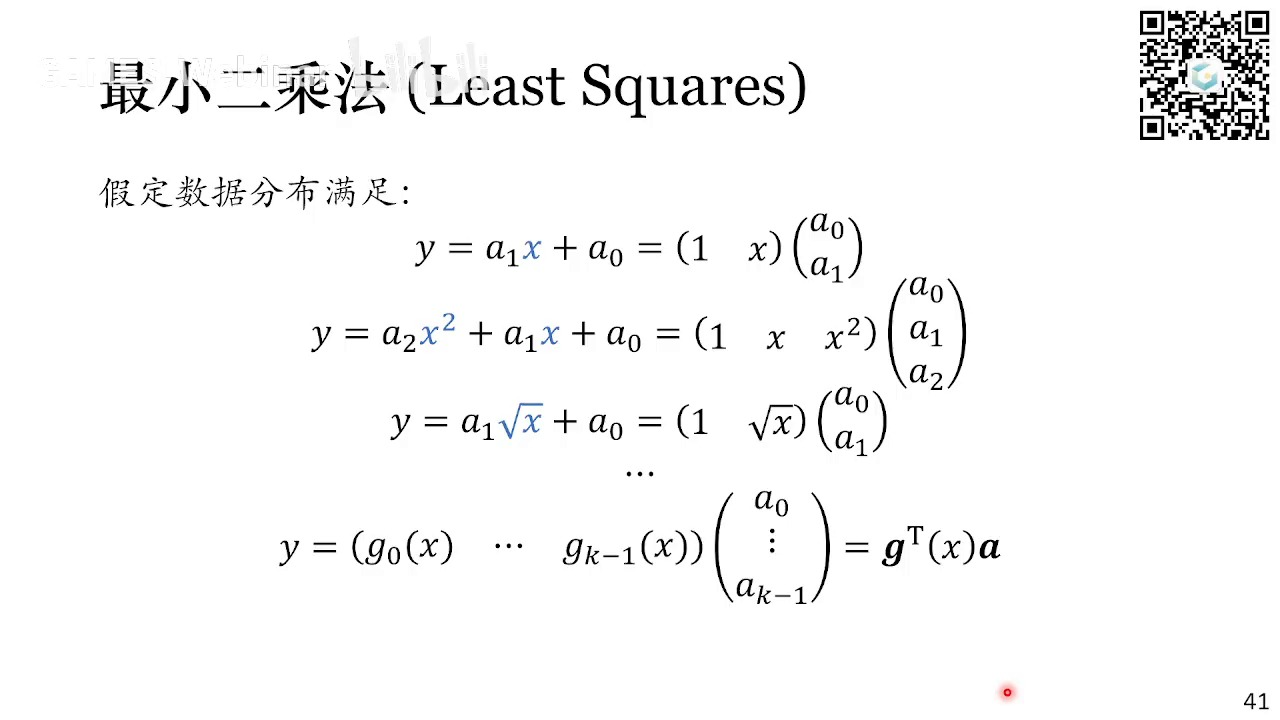
\includegraphics[width=0.92\textwidth]{figures/fig_36_lsq_model.jpg}
\caption{最小二乘法：函数对参数线性，写成 $\mathbf g^{\mathsf T}(x)\mathbf a$\vtag}
\end{figure}
\srcnote{01:10:15--01:10:30}
\end{minipage}


\noindent\begin{minipage}{\textwidth}
\begin{figure}[H]
\centering
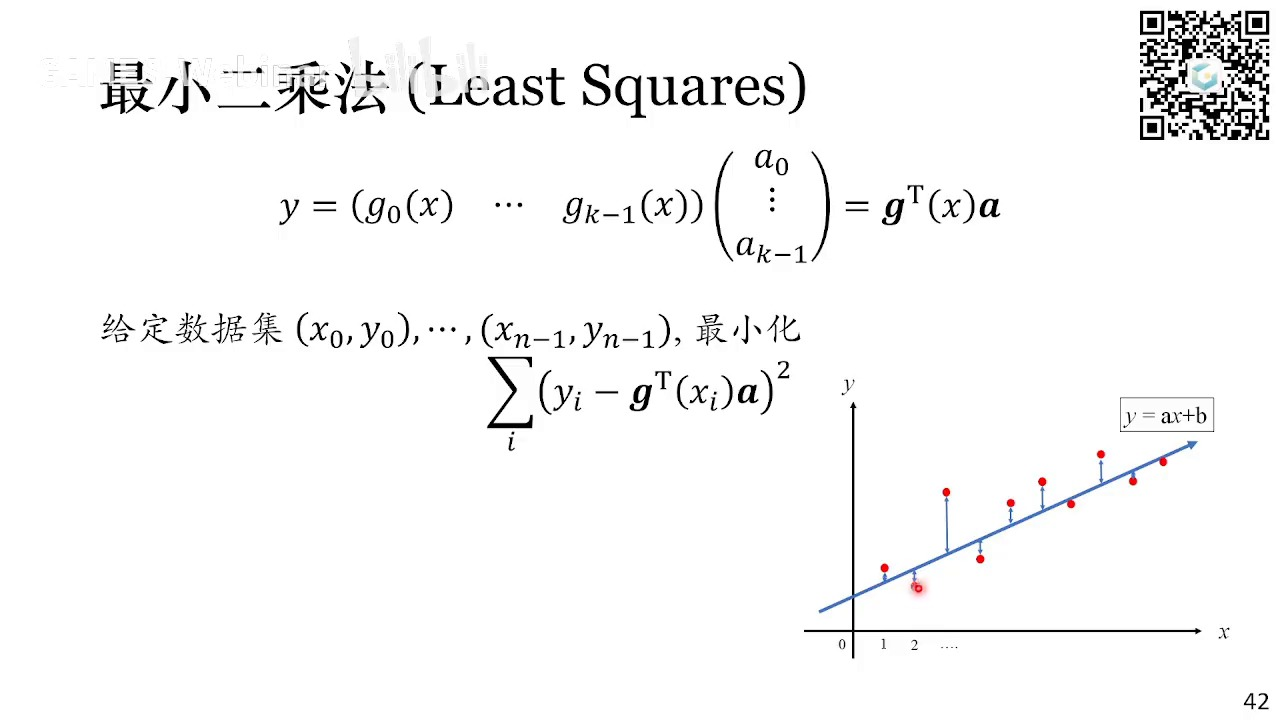
\includegraphics[width=0.92\textwidth]{figures/fig_37_lsq_objective.jpg}
\caption{最小二乘的目标：残差平方和\vtag}
\end{figure}
\srcnote{01:11:00--01:11:15}
\end{minipage}


定义矩阵 $\mathbf G\in\mathbb R^{n\times k}$，$\mathbf G_{ij}=g_j(x_i)$，以及 $\mathbf y=(y_0,\dots,y_{n-1})^{\mathsf T}$，求和就写成向量模长：
\[
\sum_i\big(y_i-\mathbf g^{\mathsf T}(x_i)\mathbf a\big)^2=\|\mathbf y-\mathbf G\mathbf a\|^2,\qquad
\min_{\mathbf a}\|\mathbf y-\mathbf G\mathbf a\|^2\;\Longrightarrow\;\mathbf a=(\mathbf G^{\mathsf T}\mathbf G)^{-1}\mathbf G^{\mathsf T}\mathbf y .
\]
这正是上一讲 SVD 与 PCA 课件第 10 页的左逆（伪逆）。算法流程是：构造 $\mathbf G$，求解 $\mathbf a$，得到拟合函数 $y=\mathbf g^{\mathsf T}(x)\mathbf a$。这个流程不光适用于最简单的一维直线拟合，也适用于高维的多项式曲面拟合。讲者建议大家用矩阵乘法推一推，看看直线拟合的结果是否和高中学过的公式等价。

\noindent\begin{minipage}{\textwidth}
\begin{figure}[H]
\centering
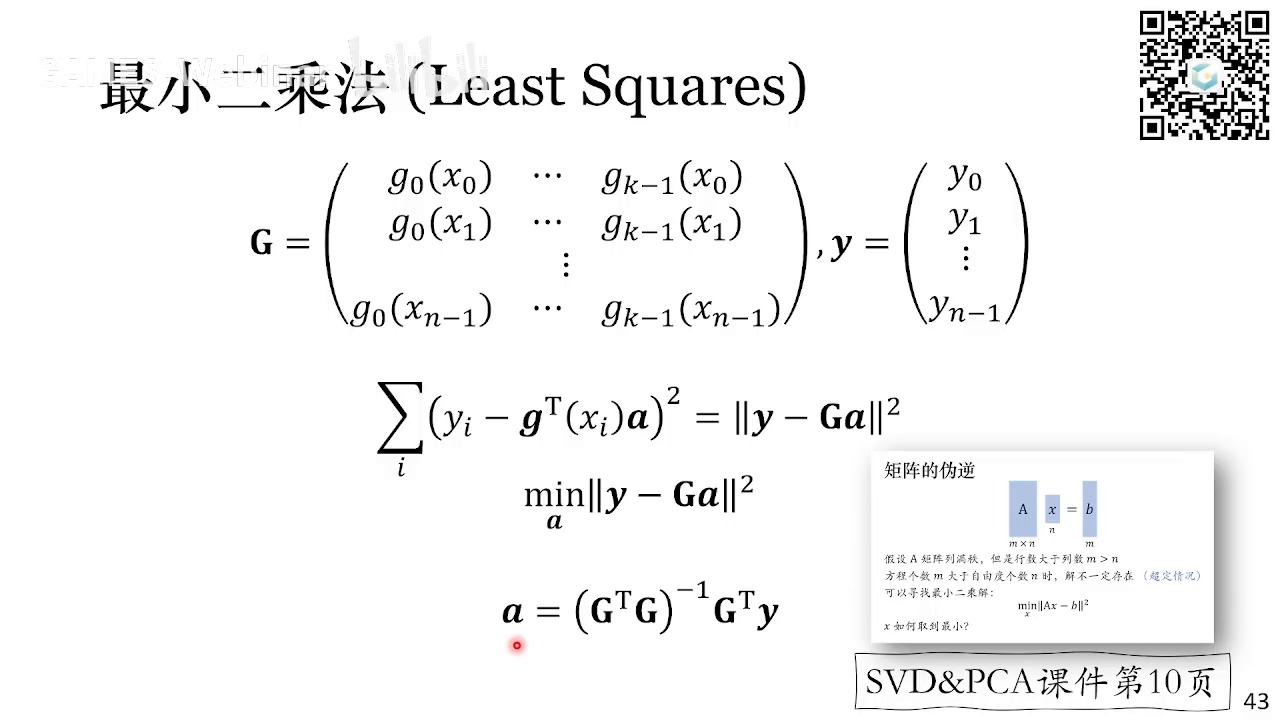
\includegraphics[width=0.92\textwidth]{figures/fig_38_lsq_matrix.jpg}
\caption{最小二乘的矩阵形式：$\mathbf a=(\mathbf G^{\mathsf T}\mathbf G)^{-1}\mathbf G^{\mathsf T}\mathbf y$\vtag}
\end{figure}
\srcnote{01:13:45--01:14:00}
\end{minipage}


\noindent\begin{minipage}{\textwidth}
\begin{figure}[H]
\centering
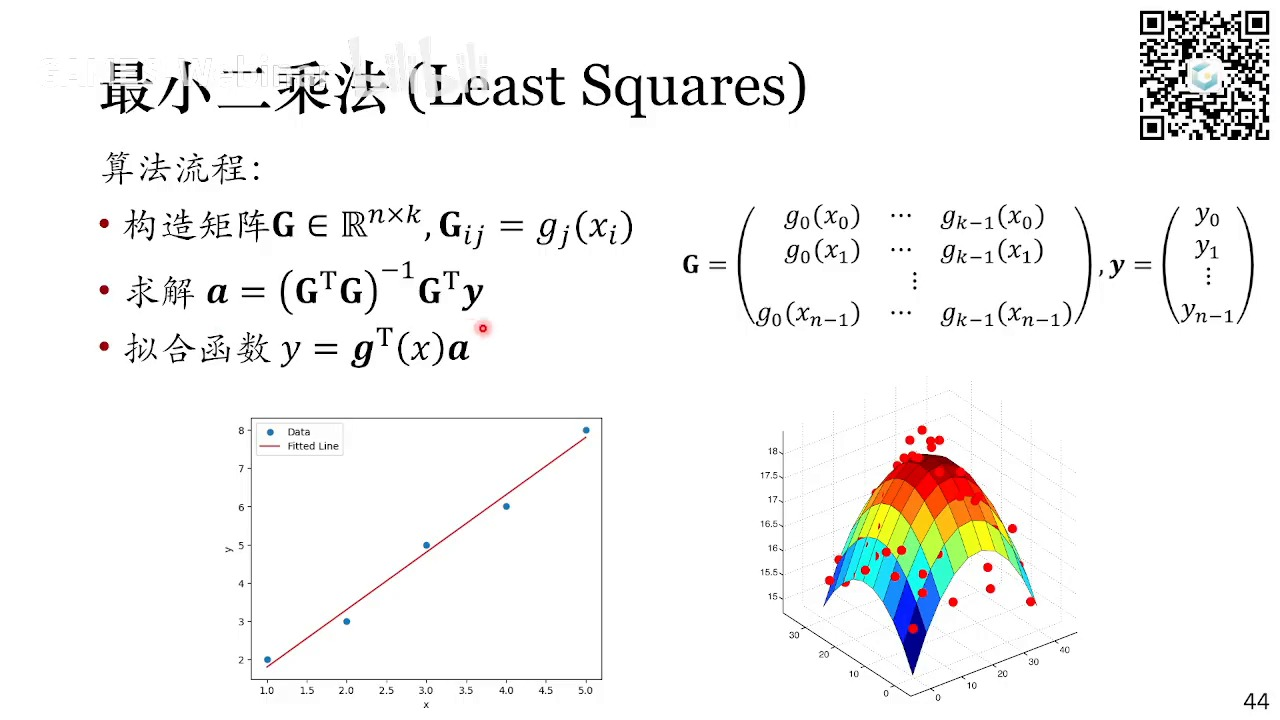
\includegraphics[width=0.92\textwidth]{figures/fig_39_lsq_algo.jpg}
\caption{最小二乘的算法流程及二维曲面拟合示例\vtag}
\end{figure}
\srcnote{01:15:00--01:15:15}
\end{minipage}


\begin{practicebox}{动手验证}
对直线 $y=a_1x+a_0$，$\mathbf G$ 的第 $i$ 行是 $(1,x_i)$。写出 $\mathbf G^{\mathsf T}\mathbf G=\begin{pmatrix}n&\sum x_i\\ \sum x_i&\sum x_i^2\end{pmatrix}$ 和 $\mathbf G^{\mathsf T}\mathbf y=\begin{pmatrix}\sum y_i\\ \sum x_iy_i\end{pmatrix}$，解出 $a_1$，与高中教材中的回归直线斜率公式 $\frac{\sum(x_i-\bar x)(y_i-\bar y)}{\sum(x_i-\bar x)^2}$ 比较。
\end{practicebox}

\subsection{移动最小二乘}

当数据整体并不服从一个简单的规律时，可以用\textbf{移动最小二乘}（moving least squares, MLS）：只在局部做多项式的最小二乘拟合；对局部的点施加权重，距离近的权重大，距离远的权重小；每当需要 $x$ 点处的值时，就以 $x$ 为中心重新做一次拟合。例如要求 $x=0.5$ 处的拟合值，就只考虑它周围的采样点；要求 $0.75$ 处的值，就在 $0.75$ 附近重新找邻近点拟合。

\noindent\begin{minipage}{\textwidth}
\begin{figure}[H]
\centering
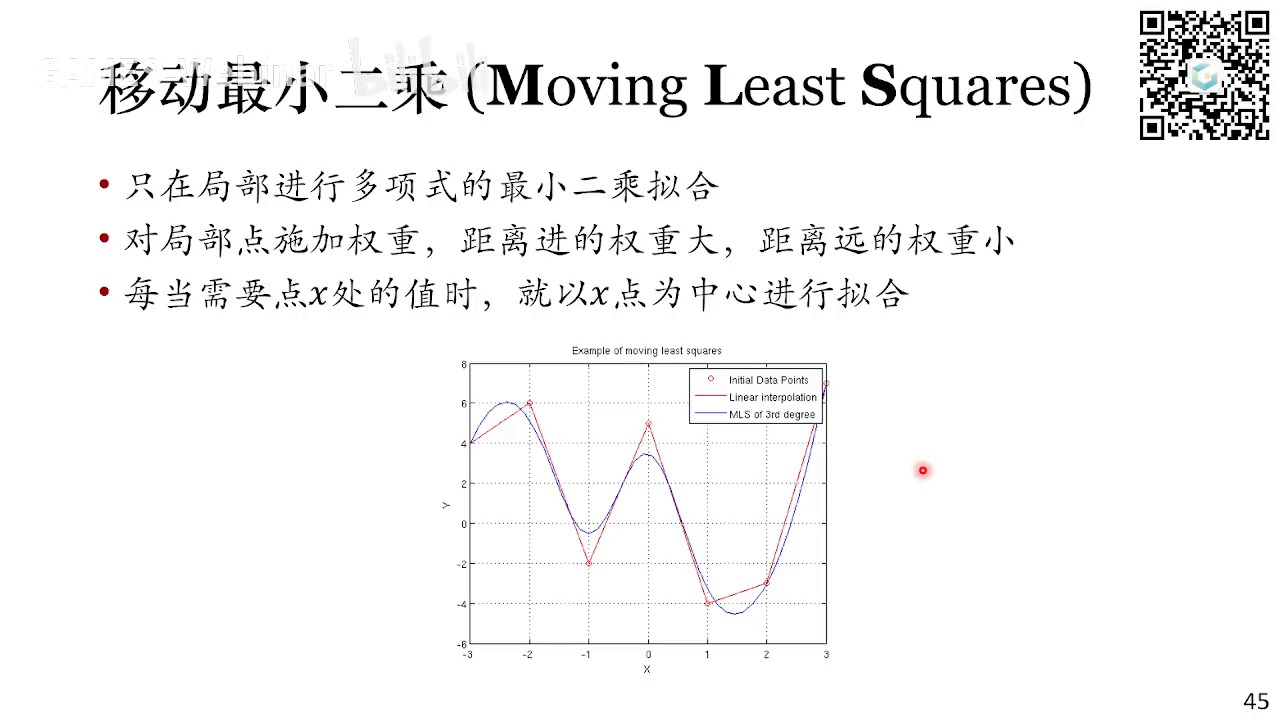
\includegraphics[width=0.92\textwidth]{figures/fig_40_mls_idea.jpg}
\caption{移动最小二乘：以待求点为中心做加权的局部拟合\vtag}
\end{figure}
\srcnote{01:17:45--01:18:00}
\end{minipage}


具体地，设 $x$ 点邻域内有 $n$ 个点 $x_0,\dots,x_{n-1}$，函数值为 $f_0,\dots,f_{n-1}$。计算相对 $x$ 的偏移 $r_i=x_i-x$，认为邻域内数据满足 $p$ 阶多项式
\[
f(r)=\begin{pmatrix}1&r&\cdots&r^p\end{pmatrix}\begin{pmatrix}a_0\\a_1\\ \vdots\\a_p\end{pmatrix}=\mathbf p^{\mathsf T}(r)\,\mathbf a .
\]
注意多项式以 $r$ 为自变量，所以 $f(0)=a_0$ 就是 $x$ 点处的拟合值，而不是 $f(x)$；并且 $f'(0)=a_1$ 对应 $x$ 点的斜率，$\frac12f''(0)=a_2$ 与 $x$ 点的曲率相关。讲者说一般取到二阶就够了，因为曲率通常是我们想要的最高阶信息。

\begin{warningbox}{$f(0)$ 才是拟合值}
初学者很容易把局部多项式直接在 $x$ 处求值，写成 $f(x)$。但这里的多项式是以偏移 $r=x_i-x$ 为自变量定义的，待求点对应 $r=0$，所以拟合值是 $f(0)=a_0$。每换一个待求点，偏移和权重都随之改变，需要重新解一次 $\mathbf a$；不能把某一点拟合出的多项式拿去别处求值。
\end{warningbox}

\noindent\begin{minipage}{\textwidth}
\begin{figure}[H]
\centering
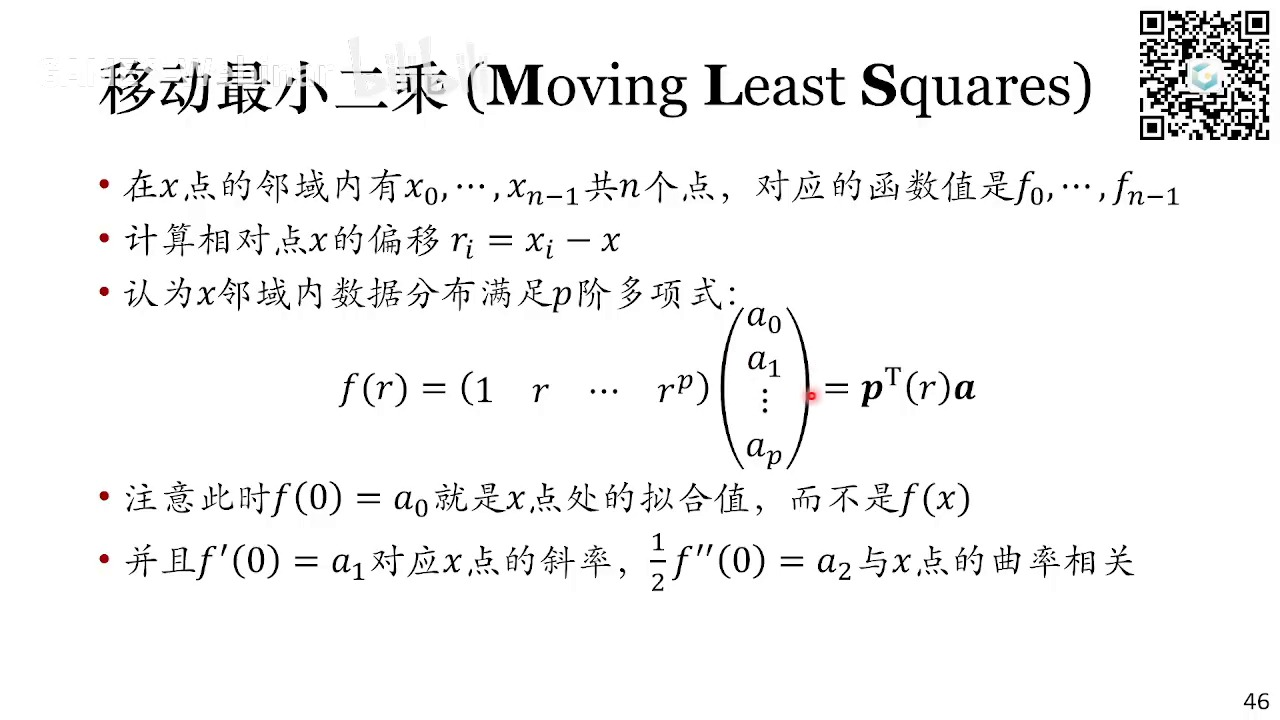
\includegraphics[width=0.92\textwidth]{figures/fig_41_mls_local.jpg}
\caption{移动最小二乘的局部多项式：$a_0$ 是拟合值，$a_1$ 是斜率，$a_2$ 与曲率相关\vtag}
\end{figure}
\srcnote{01:21:00--01:21:15}
\end{minipage}


对二维数据 $\mathbf r=(r_x,r_y)$，多项式中会出现混合项：一阶时 $\mathbf p^{\mathsf T}(\mathbf r)=(1,r_x,r_y)$，二阶时 $\mathbf p^{\mathsf T}(\mathbf r)=(1,r_x,r_y,r_x^2,r_xr_y,r_y^2)$。此时同样有 $f(\mathbf 0)=a_0$ 是拟合值，$\nabla f(\mathbf 0)=(a_1,a_2)$ 是 $\mathbf x$ 处的梯度。

\noindent\begin{minipage}{\textwidth}
\begin{figure}[H]
\centering
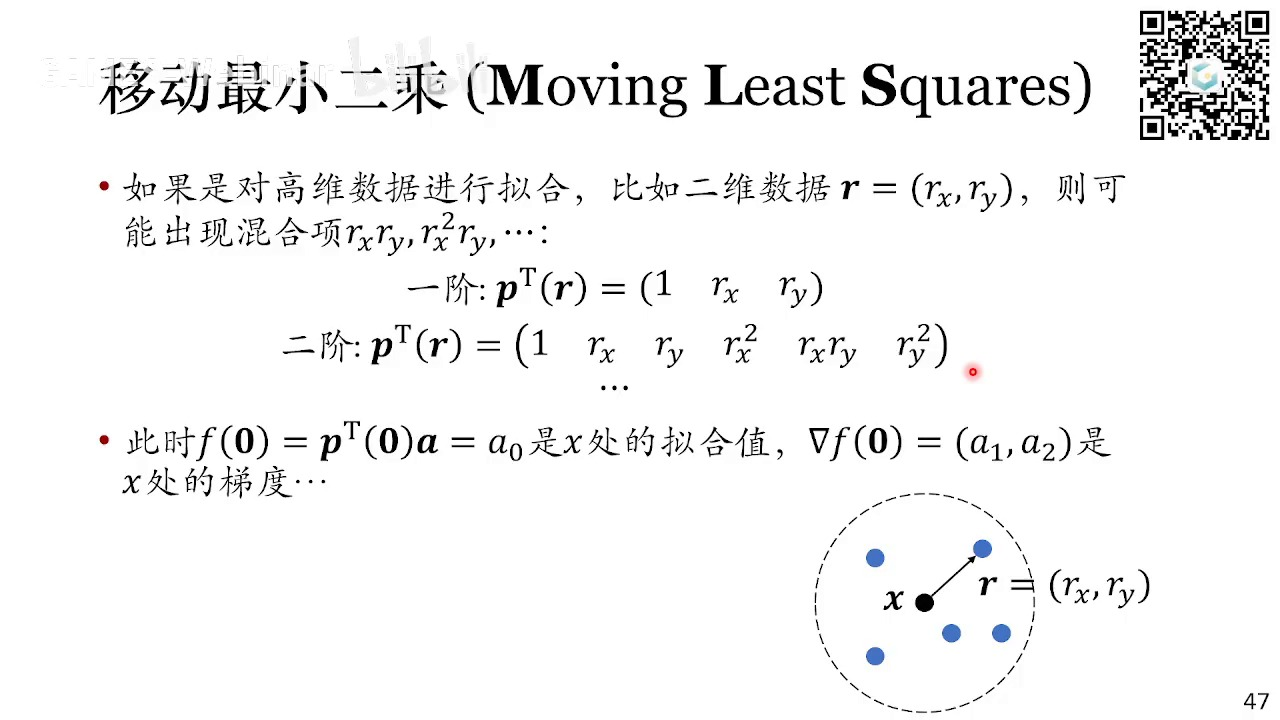
\includegraphics[width=0.92\textwidth]{figures/fig_42_mls_2d.jpg}
\caption{二维移动最小二乘：多项式中出现混合项，$\nabla f(\mathbf 0)=(a_1,a_2)$\vtag}
\end{figure}
\srcnote{01:24:00--01:24:15}
\end{minipage}


最小化的目标是加权残差平方和
\[
J=\sum_i\big(\mathbf p^{\mathsf T}(r_i)\mathbf a-f_i\big)^2\,w(r_i),
\]
其中 $w(r)$ 是权重函数，前面点云插值中提到的高斯核、拉普拉斯核、二次有理核都可以使用：$r_i$ 大，权重小；$r_i$ 小，权重大。权重不需要归一化，因为所有权重同乘一个常数只会让 $J$ 整体放大，不影响最小值的位置。令 $\partial J/\partial\mathbf a=0$，得到
\[
\mathbf M=\sum_iw(r_i)\,\mathbf p(r_i)\mathbf p^{\mathsf T}(r_i),\qquad
\mathbf b=\sum_iw(r_i)\,f_i\,\mathbf p(r_i),\qquad
\mathbf a=\mathbf M^{-1}\mathbf b .
\]
$\mathbf M$ 的维数等于未知数的个数，即 $\mathbf a$ 的维数：一维二阶时是 $3\times3$，二维二阶时是 $6\times6$，都很小。解出的 $\mathbf a$ 里同时包含了该点的函数值和导数信息，二阶时还有曲率信息。所以移动最小二乘名字上和最小二乘关系很大，用起来却更像一种插值方法。

\noindent\begin{minipage}{\textwidth}
\begin{figure}[H]
\centering
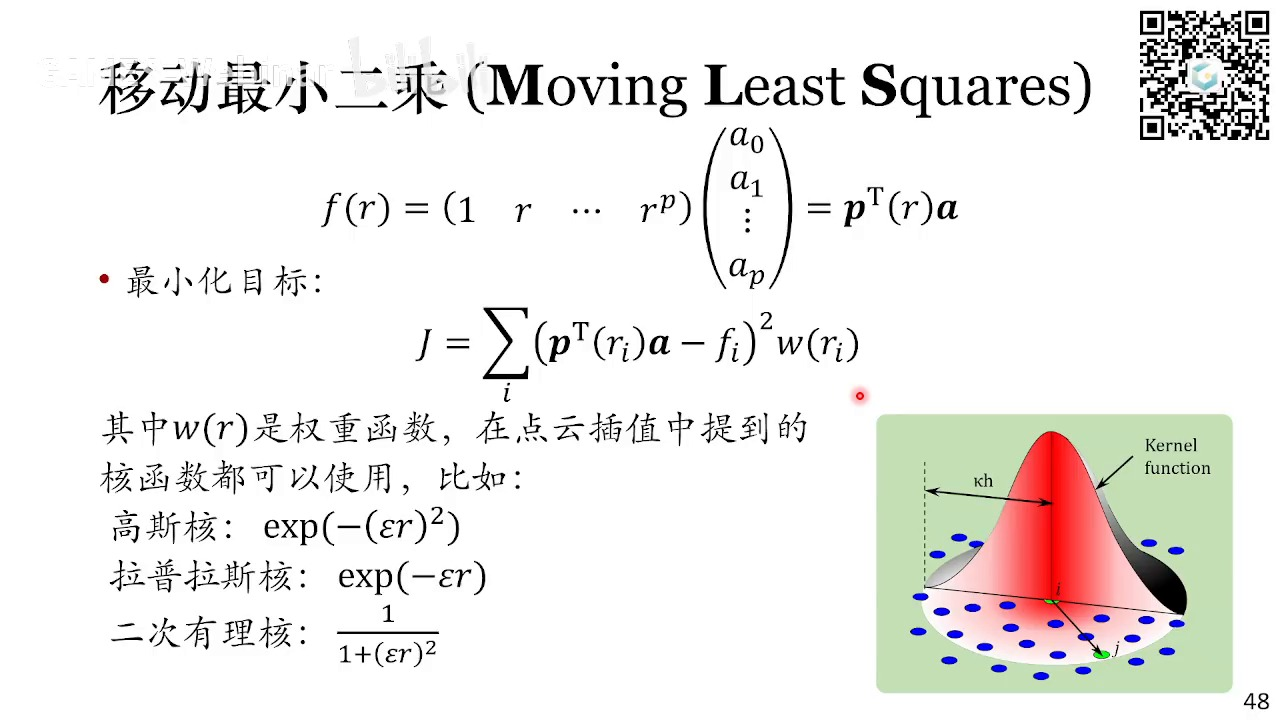
\includegraphics[width=0.92\textwidth]{figures/fig_43_mls_objective.jpg}
\caption{移动最小二乘的加权目标函数与核函数权重\vtag}
\end{figure}
\srcnote{01:26:15--01:26:30}
\end{minipage}


\noindent\begin{minipage}{\textwidth}
\begin{figure}[H]
\centering
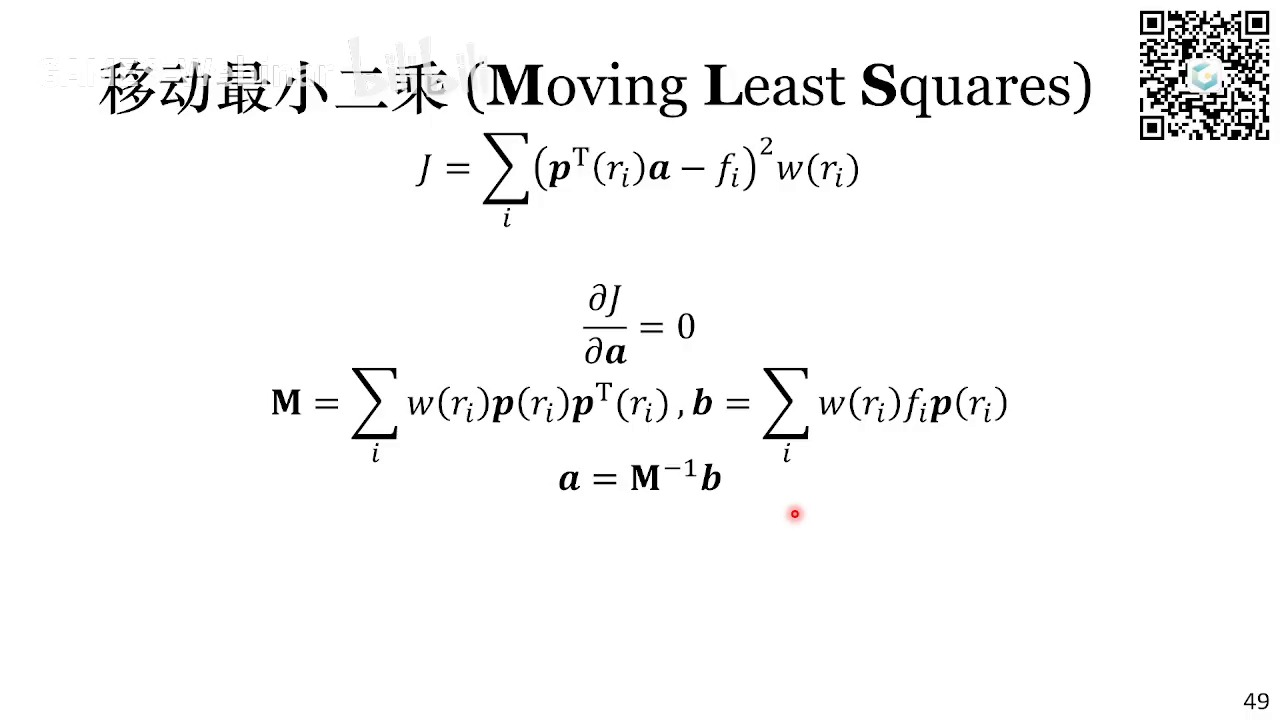
\includegraphics[width=0.92\textwidth]{figures/fig_44_mls_solve.jpg}
\caption{移动最小二乘的求解：$\mathbf a=\mathbf M^{-1}\mathbf b$\vtag}
\end{figure}
\srcnote{01:28:15--01:28:30}
\end{minipage}


\subsection{RANSAC}

最小二乘假设所有数据都“有用”，只是带有噪声。如果数据集中有大量离群点，它们会把拟合结果拉偏。RANSAC（random sample consensus）适用于这种情况：我们想把有用的数据囊括进来做拟合，而把不想要的噪声剔除掉、根本不予考虑。它的算法很符合直觉：

\begin{enumerate}
\item 从数据集中随机选择 $n$ 个点拟合直线；
\item 把剩下的点分为两类：到拟合直线距离小于 $t$ 的是内点，大于 $t$ 的是外点；
\item 如果内点数量大于等于 $d$，就用所有内点重新拟合，并终止算法；
\item 否则说明这条直线还没有落在想要的分布上，重新选点，重复上面的过程。
\end{enumerate}

\noindent\begin{minipage}{\textwidth}
\begin{figure}[H]
\centering
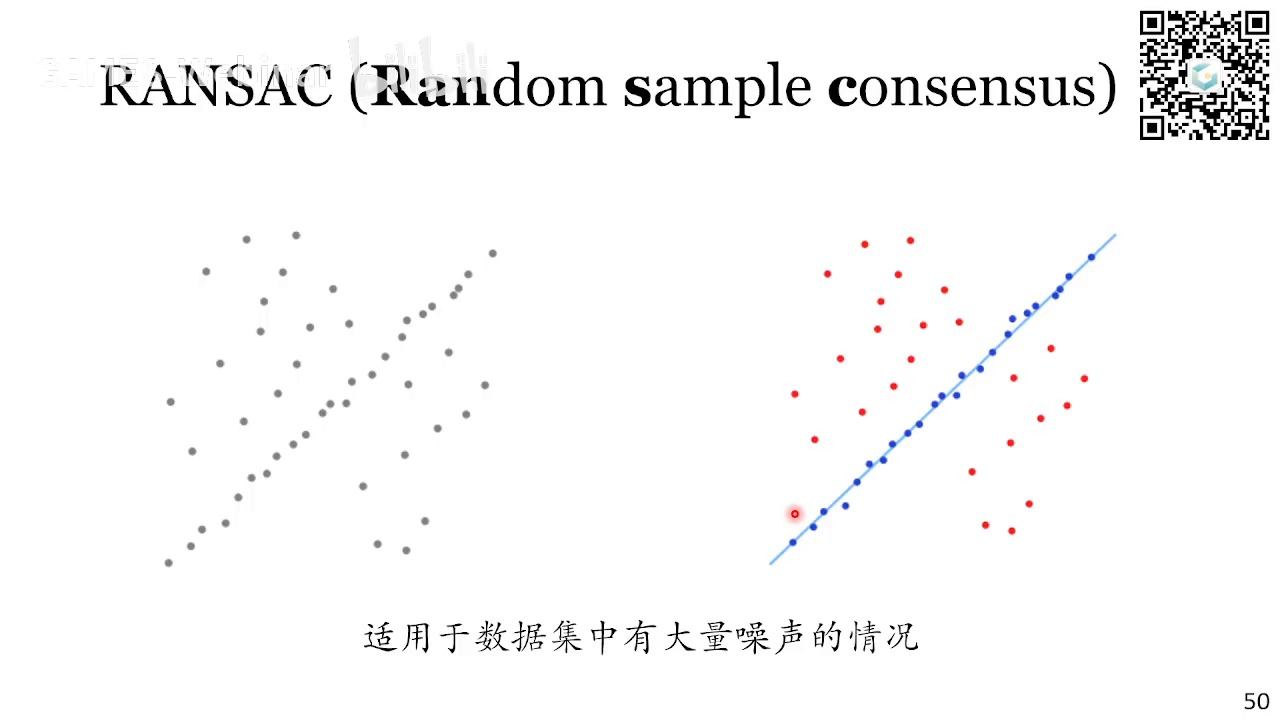
\includegraphics[width=0.92\textwidth]{figures/fig_45_ransac_data.jpg}
\caption{RANSAC 适用于数据集中有大量噪声的情况\vtag}
\end{figure}
\srcnote{01:29:15--01:29:30}
\end{minipage}


\noindent\begin{minipage}{\textwidth}
\begin{figure}[H]
\centering
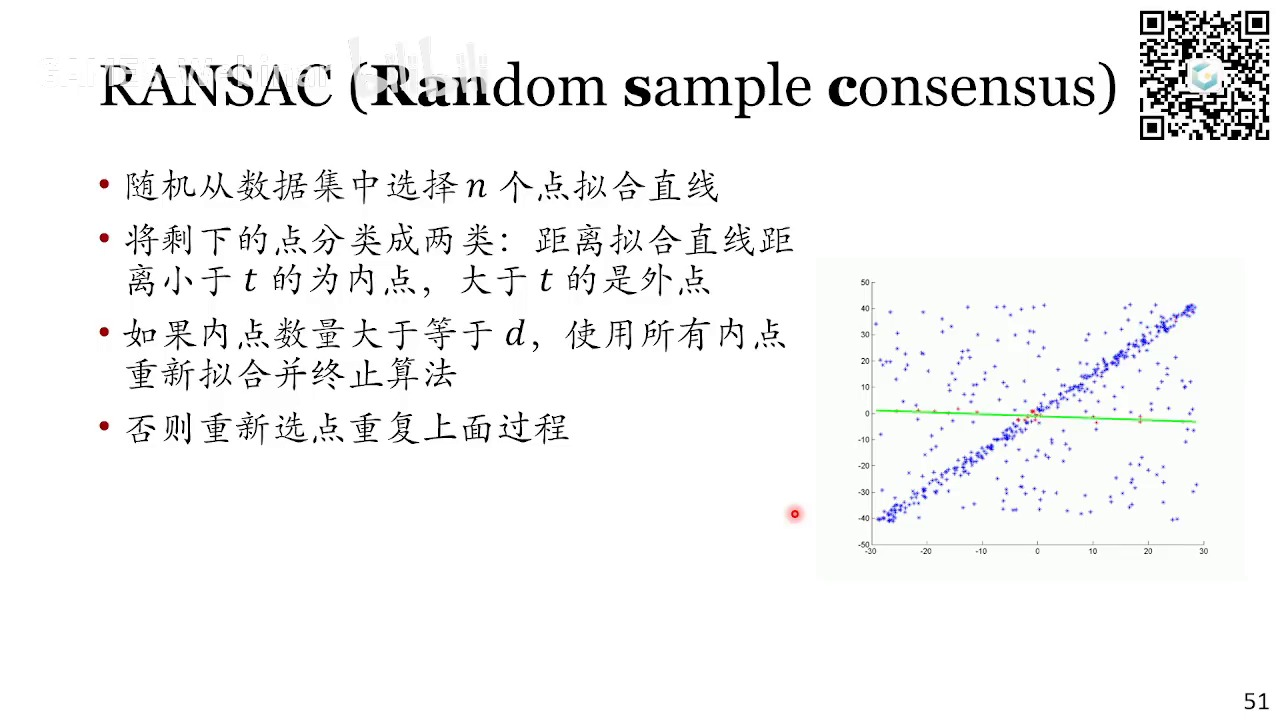
\includegraphics[width=0.92\textwidth]{figures/fig_46_ransac_algo.jpg}
\caption{RANSAC 算法：随机采样拟合、区分内外点、按内点数判断\vtag}
\end{figure}
\srcnote{01:30:45--01:31:00}
\end{minipage}


\begin{warningbox}{RANSAC 的参数}
讲义作者补充：RANSAC 的效果取决于三个参数：每次采样的点数 $n$（拟合直线取 2 即可）、内点阈值 $t$ 和接受阈值 $d$。若内点比例为 $w$，一次采样全是内点的概率为 $w^n$，要以概率 $p$ 至少成功一次，需要的迭代次数约为 $\log(1-p)/\log(1-w^n)$。离群点越多、$n$ 越大，需要的迭代次数增长越快。
\end{warningbox}

\section{总结与作业}

这一讲的作业只有一道题，讲者说不必有大的压力：推导三阶厄米样条插值的基函数，它是本讲中最重要、应用最广泛的插值方法。课后有同学反馈作业二和作业三提交时文件类型多了一个星号，助教表示会处理。

\begin{practicebox}{自测清单}
\begin{itemize}
\item 区分插值与拟合，并各举一个图形学中的例子。
\item 证明拉格朗日多项式满足 $L_j(x_k)=\delta_{jk}$，并解释龙格现象的成因。
\item 数一数二阶、三阶样条的未知数和方程个数，说明还需要几个额外条件。
\item 从 $y(0),y(1),y'(0),y'(1)$ 四个条件推导厄米基函数 $h_{00},h_{10},h_{01},h_{11}$（本讲作业）。
\item 用基函数的视角说明为什么 $B_i(x_j)=\delta_{ij}$ 就能保证插值条件。
\item 写出 RBF 插值的线性方程组，并说明 SPH、3DGS 为什么不需要解这个方程。
\item 推导移动最小二乘的 $\mathbf a=\mathbf M^{-1}\mathbf b$，说明 $a_0,a_1,a_2$ 的含义。
\end{itemize}
\end{practicebox}

\end{document}
